% LaTeX-Vorlage zur Erstellung von Abschlussarbeiten an der FH Aachen
% Author: Sven Hinz
% Aenderung für FB 5: Ingo Elsen

\documentclass[12pt,a4paper, oneside]{scrreprt}
% Paket für Umlaute:
\usepackage[utf8]{inputenc}       % Cross Platform
%\usepackage[ansinew]{inputenc}   % Windows
%\usepackage[latin1]{inputenc}    % Linux
%\usepackage[applemac]{inputenc}  % Mac

\usepackage[ngerman]{babel}       % Sprache: deutsch
\usepackage[utf8]{inputenc} % For degree symbol in tex source
\usepackage{amsmath}
\usepackage{amsfonts}
\usepackage{amssymb}
\usepackage{makeidx}
\usepackage{graphicx}
\usepackage{epstopdf}
%\usepackage{kpfonts}
\usepackage{textcomp}
\usepackage[left=3cm,right=3cm,top=2.5cm,bottom=2.5cm]{geometry}
\usepackage[plainheadsepline,headsepline]{scrlayer-scrpage}
\usepackage{color}
\usepackage{setspace}
%\usepackage[numbers,square]{natbib} % only required for unsrtd bib style
\usepackage{longtable}
\usepackage{listings}
\usepackage{rotating}
\usepackage{pdfpages}
\usepackage{caption}
\usepackage{subcaption}
\parindent 0pt
\usepackage{booktabs}
\usepackage[export]{adjustbox}



% Schriftart
\usepackage{courier}
\usepackage{helvet}
\usepackage{times}
%\renewcommand{\familydefault}{\sfdefault}
\renewcommand{\familydefault}{\rmdefault}
\setkomafont{chapter}{\sffamily \large}
\setkomafont{section}{\sffamily \normalsize}
\setkomafont{subsection}{\sffamily \normalsize}
\setkomafont{subsubsection}{\sffamily \normalsize}
\addtokomafont{caption}{\sffamily \small}


% Abstand zwischen Kopfzeile und Kapitelüberschrift
\renewcommand*{\chapterheadstartvskip}{\vspace*{-0.75\baselineskip}}

% Einstellungen der Kopf- und Fußzeile
\pagestyle{scrheadings}
%\ihead[\sffamily \bfseries \upshape \headmark]{\sffamily \bfseries \upshape \headmark}
\ohead[\sffamily \bfseries \upshape \headmark]{\sffamily \bfseries \upshape \headmark}
\chead[]{}
%\ohead[]{}
\ifoot[]{}
\cfoot[]{}
\ofoot[\sffamily \pagemark]{\sffamily \pagemark}
\automark[]{chapter}
\renewcommand*{\chapterheadendvskip}{\vspace*{1\baselineskip}}

% Formeln
\usepackage{fleqn} % linksbündig
\setlength{\mathindent}{1.5cm} % Einrücktiefe

% Tabellen
\usepackage{multirow} % mehrzeiliger Text in einer Spalte
\renewcommand{\arraystretch}{2} % Zeilenabstand vergrößern
\setlength{\doublerulesep}{0.1mm} % Abstand der Doppellinien verkleinern
\usepackage{tabu}
\newcolumntype{C}{>{\centering\arraybackslash$}p{3cm}<{$}}

% Quellcode / Kommandozeileneingabe
\lstdefinestyle{BashInputStyle}{
  language=bash,
  basicstyle=\small\ttfamily,
  %numbers=left,
  %numberstyle=\tiny,
  %numbersep=3pt,
  frame=tb,
  columns=fullflexible,
  %backgroundcolor=\color{yellow!20},
  linewidth=0.9\linewidth,
  xleftmargin=0.1\linewidth
}

% Inhalt
\renewcaptionname{ngerman}{\contentsname}{Inhalt} % Umbenennung in Inhalt

% Quellenverzeichnis
\renewcaptionname{ngerman}{\bibname}{Quellenverzeichnis} % Umbenennung in Quellenverzeichnis


% Abkürzungsverzeichnis
%\usepackage[intoc]{nomencl}
%\let\abbrev\nomenclature
%\renewcommand{\nomname}{Abkürzungsverzeichnis}
%\setlength{\nomlabelwidth}{.25\hsize}
%\renewcommand{\nomlabel}[1]{#1 \dotfill}
%\setlength{\nomitemsep}{-\parsep}
%\makenomenclature

\usepackage[]{acronym}


\author{Vorname Nachname} % --> Eigenen Namen einfügen


\begin{document}
\setstretch{1.1}
\addtocontents{toc}{\linespread{1}}

% Einbinden der Textinhalte mit '\include{...}'
% Die Dateien mit den Textinhalten befinden sich im Ordner 'doc'

\begin{titlepage}
	%ab hier kleinere Raender, mehr bedruckbare Flaeche.
	%\fontfamily{\sffamily}\selectfont
	\thispagestyle{empty}
	\newgeometry{a4paper, portrait, left=0cm, right=0cm, top=0.6cm, bottom=0cm, includefoot}

	% FH Logo
	\begin{flushright}
		
\includegraphics[width=1.7cm]{./pic/FHAC.jpg}
	\end{flushright}

	\vspace{-2.5cm}

	% Kopfzeile mit Fachbereich ...
	\centering \sffamily \bfseries \Large FH~Aachen \\
	\vspace{0.5cm}
	\normalsize Fachbereich\\
	Elektrotechnik und Informationstechnik

	\vspace{1cm}

	\centering \bfseries Bachelorarbeit
	%\centering \bfseries Masterarbeit

	\vspace{0.8cm}

	%Titel der Arbeit
	\centering \begin{minipage}[t]{17cm}
		\centering \bfseries \large Prognose der Anwesenheit von Personen für die Gebäudeautomatisierung 
		mittels Umweltsensordaten
		\medskip
	\end{minipage}

	\vspace{1.5cm}

	%Name und Matrikelnummer
	%\vspace*{1cm}
	%\hspace*{6.8cm}
	\begin{minipage}[t]{9cm}
		\centering Alexander Loosen \\ Matr.-Nr.: 3167353
	\end{minipage}

	\vspace{2.1cm}

	%Professor und Betreuer
	%\vspace*{4.7cm}
	%\hspace*{6.8cm}
	\centering \begin{minipage}[t]{9cm}
		\centering \begin{tabular}{ll}
			Referent: & Prof. Dr-Ing. Ingo Elsen\\
			Korreferent: & M.Sc Marcel Remmy\\
			%Externer Betreuer: & Dipl.-Wirt.-Ing\\
		\end{tabular}
	\end{minipage}

	\vspace{7cm}

	% Firmenlogo
	%\begin{flushleft}
	%\centering \hspace{-8cm}
	%\begin{minipage}[t]{5cm}
			%\includegraphics[width=5cm]{./pic/firmenlogo.jpg}
	%\end{minipage}
	%\end{flushleft}


	%Erstellungsdatum
	%\vspace{-4cm}
	%\begin{flushright}
	\centering %\hspace{8cm}
	\begin{minipage}[b]{5cm}
			\centering
			\today\\ %Datum\\
			%\vspace{1cm}
			%In Zusammenarbeit mit\\
			%Firma, Ort\\
			%\vspace{1cm}
			%vertraulich bis xx.xx.xx
	\end{minipage}
	%\end{flushright}

	%\today
	\restoregeometry
\end{titlepage}


\clearpage
\chapter*{Erklärung}\label{erklaerung}
\markboth{Erklärung}{Erklärung}
Ich versichere hiermit, dass ich die vorliegende Arbeit selbstständig verfasst und keine anderen als die im Literaturverzeichnis angegebenen Quellen benutzt habe.

\bigskip

Stellen, die wörtlich oder sinngemäß aus veröffentlichten oder noch nicht veröffentlichten Quellen entnommen sind, sind als solche kenntlich gemacht.

\bigskip

Die Zeichnungen oder Abbildungen in dieser Arbeit sind von mir selbst erstellt worden oder mit einem entsprechenden Quellennachweis versehen.

\bigskip

Diese Arbeit ist in gleicher oder ähnlicher Form noch bei keiner anderen Prüfungsbehörde eingereicht worden.

\vspace{1cm}
Aachen, \today %Monat Jahr

\vspace{7cm}
\section*{Geheimhaltung - Sperrvermerk}\label{geheimhaltung}

Die vorliegende Arbeit unterliegt bis zum 25.04. der Geheimhaltung. Sie darf vorher weder vollständig noch auszugsweise ohne schriftliche Zustimmung des Autors oder des betreuenden Referenten vervielfältigt, veröffentlicht oder Dritten zugänglich gemacht werden.

%\clearpage
\chapter*{Danksagung}\label{danksagung}
\markboth{Danksagung}{Danksagung}
Danke.

% Inhaltsverzeichnis
\clearpage
\makeatletter
\renewcommand*{\@dotsep}{1} % Punktabstand einstellen
\makeatother
\tableofcontents

% Das erste Kapitel soll auf einer ungeraden Seite beginnen.
\cleardoublepage
\setstretch{1.1}

% Nicht benötigte Kapitel können auskommentiert werden
% Für zusätzliche Kapitel müssen weitere Dateien im Ordner 'doc' angelegt werden

\clearpage
\chapter{\textbf{Einleitung}}\label{einleitung}
%\addtocontents{toc}{\vspace{0.8cm}}


%\par\medskip

Gebäudeautomatisierung bezeichnet die automatische Steuerung und Regelung von Ge-bäudetechnik 
wie Heizung, Lüftung oder Beleuchtung. Während sie bisher hauptsächlich für die Optimierung 
der Energieeffizienz von gewerblichen und öffentlichen Gebäuden genutzt wurde, welche in 
Zuge solcher Optimierungsschritte als ,,Smart Buildings'' bezeichnet werden, 
rückt sie in den letzten Jahren zunehmend unter dem Begriff ,,Smart Home'' auch in den privaten 
Bereich.\\
Die beiden Begriffe stehen in den letzten Jahren so im Vordergrund, weil eine
Verbesserung der Energieeffizienz durch bauphysikalische Maßnahmen, wie verminderte 
Wärmeverluste durch bessere Isolation, an ihre Grenzen gestoßen sind.
\\\\
In Deutschland haben private Haushalte einen Anteil am gesamten Energieverbrauch des Landes von 
etwa 30\%. Davon nimmt die Erzeugung der Raumwärme einen Anteil von etwa 70\% ein. Vorallem bezogen
auf den Energieverbrauch durch das Heizen stellt die Gebäudeautomatisierung also einen der größten
Sektoren dar, in denen eine Optimierung der Prozesse entscheidend wäre. Beispielsweise können Wärmeverluste
über die Nacht hinweg um 20\% verringert werden, wenn Abends die Rolläden heruntergelassen werden.\\\\
Zur weiteren Steigerung der Energieeffizienz ist es also nötig, die Gebäudetechnik insofern
automatisch anzusteuern, sodass sog. Performance-Gaps vermieden werden. Performance-Gaps
stellen eine Diskrepanz im Energieverbrauch eines Gebäudes zwischen einem theoretischen 
Soll-Wert zu einem tatsächlichem Ist-Wert dar.\\


\section{Motivation und Aufgabenstellung}
%\addtocontents{toc}{\vspace{0.8cm}}

Für nahezu alle Bereiche der Gebäudeautomatisierung stellt die Anwesenheit 
von Personen eine zentrale Variable dar. Es ist entscheidend bei einem Optimierungsprozess zu erkennen, zu
welchen Zeitpunkten sich Menschen in einem Raum aufhalten. Beispielsweise werden in vielen gewerblich 
genutzen Gebäuden werden grundsätzlich alle Räume beheizt - unabhängig von tatsächlicher Anwesenheit von Personen. 
Eine Erkennung von menschlicher Anwesenheit ist bei der Optimierung also essenziell.\\\\
Da die direkte Messung von Anwesenheit über z.B. Infrarot- oder Kamerasensoren rechtlich problematisch ist, 
soll in dieser Arbeit untersucht werden, inwiefern Machine-Learning Algorithmen genutzt werden können, 
um eine genaue Erwartung über die Anwesenheit von Personen anhand von CO2-Werten in der Raumluft zu treffen.\\\\
Die Motivation der Optimierung der Gebäudeautomatisierung exisitert, da ein steigender CO2-Gehalt der 
Raumluft nachweislich mit einer Abnahme der menschlich kognitiven Leistung einhergeht. Mehrere Studien
konnten belegen, dass sowohl sprachliche als auch logisch- mathematische Fähigkeiten abnehmen, sobald 
der CO2-Gehalt der  Raumluft bestimmte Werte überschreitet.\\ 
Um eine angemessene Datengrundlage zu schaffen, wurden in diversen Büro-Räumen der FH Aachen Temperatur-,
Luftfeuchtigkeits-, Infrarot- und CO2-Sensoren angebracht, deren Messungen kontinuierlich auf einer Datenbank
gespeichert wurden. Der Zeitraum der Messwerte begann Mitte 2021.\\
In allen Räumen sind täglich ein oder mehrere
Personen im Rahmen eines ca. 8 stündigen Arbeitstages anwesend, weshalb die Temperatur-, Luftfeuchtigkeits-
und CO2-Werte als aussagekräftige Indikatoren für menschliche Präsenz angesehen werden können.
Es gab keine Einschränkungen hinsichtlich dessen, welche konkreten Machine-Learning Algorithmen 
benutzt werden sollten.\\\\
Als Programmiersprache für das Projekt wurde Python gewählt. Python ist wegen seiner umfassenden
Machine-Learning Bibliotheken und einfachen Auswertungstechniken anhand von z.B. Graphen und Statistiken 
gut für diesen Anwendungsfall geeignet.



%% Beispiel für das Einfügen einer Abbildung

%\begin{figure}[h]
%	\centering
%		\includegraphics[width=0.8\textwidth]{pic/dateiname.png}
%	\caption{Beispielbild}
%	\label{fig:beispielbild}
%\end{figure}
%\vspace{7cm} % Abstand unter dem Bild


\newpage

\section{Vorgehensweise}
%\addtocontents{toc}{\vspace{0.8cm}} % -> Abstand im Inhaltsverzeichnis

% Untersuchungsverlauf(pro Kapitel ein kurzer Absatz mit Verweis auf die Kapitelnummer)

Das Projekte beschäftigte sich im Schwerpunkt mit den folgenden Arbeitsschritten:
\begin{itemize}
    \item Datenbeschaffung durch Datenbankzugriffe per SQL
    \item Analyse und Vorbereitung der Daten (Pre-Processing)
    \item Trainieren von Machine-Learning Models anhand der vorbereiteten Datensets
    \item Ergebnisauswertung durch Gegenüberstellung verschiedener Datensets und Models
\end{itemize}
Da es zwischen allen verfügbaren Datensets der einzlnen Räume und Machine-Learning-Models eine Vielzahl an
Kombinationsmöglichkeiten gibt, war es ein Anspruch der Projektarbeit, ein möglichst übersichtliches, 
gut gekapseltes Python Programm zu erstellen, mit dem man einfach und schnell verschiedene Datensets  
verarbeiten und mit einer dem Forschungszweck angemessenen Anzahl von Machine-Learning Models auszuwerten. \\\\
Um einen Vergleich der Ergebnisse zu ermöglichen, sollen diese klar und verständlich dargestellt werden. 
Da nicht bei allen Algorithmen die gleichen Leistungsindikatoren genutzt werden, sollen hauptsächlich nur 
jene Indikatoren betrachtet werden, die bzgl. aller Algorithmen auch gleiche Bedeutung haben. Falls Model-
spezifische Leistungsindikatoren als besonders Erkenntnisreich erachtet werden, wird dies in dieser Arbeit
angemerkt. % Einleitung
\clearpage
\chapter{\textbf{Stand der Technik für Anwesenheitserkennung/-prognose}}\label{grundlagen}
%\addtocontents{toc}{\vspace{0.5cm}}

Man kann verschiedene Techniken zur Anwesenheitserkennung und -prognose in Innenräumen in \textit{aktive} und
\textit{passive} Verfahren unterteilen. \\\\
%\section{Aktive und Passive Messverfahren}
Aktive Verfahren messen die menschliche Anwesenheit etwa mit 
Kamera- oder Infrarotsensoren, welche den Menschen direkt im Raum erkennen können. Ein Kamerasensor nimmt
dabei kontinuierlich Bilder des Raumes auf, während ein Algorithmus im Hintergrund versucht ein 3D-Modell 
eines menschlichen Skeletts auf sich bewegende Teile des Bildes zu legen. Bewegen sich über mehrere Bilder 
hinweg die Bereiche auf und unmittelbar neben dem 3D-Modell, registriert das System eine Anwesenheit.\\\\
Infrarotsensoren dagegen funktionieren eher wie ein klassischer Bewegungsmelder, welcher Unterschiede in der 
Infrarotstrahlung eines Raumes erkennt. Durch die generierte Körperwärme des menschlichen Körpers verursacht 
ein Mensch, der sich durch den Sensor bewegt, einen Ausschlag des Sensors.\\

Passive Verfahren orientieren sich an den physikalischen Eigenschaften des Raumes. Anstatt die Präsenz des 
Menschen direkt zu messen, wird versucht, diese anhand von Veränderungen der Eigenschaften der Raumluft oder 
elektromagnetischer Strahlung des Raumes zu erkennen. \\
Verändert sich beispielsweise durch menschliche Anwesenheit die Luftfeuchtigkeit 
in einem Raum in sehr geringem Maß, wird die  Laufzeit einer Ultraschallwelle, die durch diesen Raum 
geschickt wird, leicht verringert, da die Schallgeschwindigkeit in dichteren Medien zunimmt.\\
Die Systeme unterscheiden sich neben der Art der Messung auch deutlich in der Komplexität der Implementierung.
Während Ultraschallsensoren wegen der verhältnismäßig geringen Schallgeschwindigkeit keine besonders hohe 
Genauigkeit besitzen müssen, sind die an einen Mikrowellensensor gestellten Ansprüche wesentlich höher, da sich
Mikrowellen mit deutlich höherer Geschwindigkeit im Raum ausbreiten. Mikrowellen erreichen in Atemluft Geschwindigkeiten
von ca. $300\cdot10^6 \,m/s$, Schallwellen lediglich ca. $330\, m/s$.
Mit Mikrowellen können Bewegungen durch Ausnutzung des Doppler-Effektes einer elektromagnetischen Welle erkannt 
werden. Bewegen sich Objekte oder Personen auf den Sensor zu, wird das Echo der Welle gestaucht, wodurch die 
Bewegung erkannt wird.\\
Hier verdeutlicht sich nochmals die Motivation dieser Arbeit, da Sensoren für Temperatur, Luftfeuchtigkeit oder CO2
weder teuer sind, noch besondere Ansprüche an Positionierung im Raum oder Kalibrierung besitzen.

\chapter{\textbf{Untersuchte Verfahren}}

\section{Machine Learning}\label{unterkapitel}
\addtocontents{toc}{}%\vspace{0.8cm}}

Machine Learning ist ein Teilbereich der künstlichen Intelligenz und beschreibt das Entwickeln mathematischer 
Modelle zur statistischen Auswertung von Daten.\\
Dabei wird dem Modell anhand von Trainingsdaten beigebracht, Gesetzmäßigkeiten zu erkennen, um danach Erwartungen 
über bisher unbekannte Daten treffen zu können.  
Beispielsweise könnte ein solches Modell aus einem Datenset mit aktueller Jahreszeit, Uhrzeit und 
Position der Sonne am Himmel trainiert werden, sodass es schließlich auch in einem anderen Datenset 
aus Jahreszeit und Position der Sonne Rückschlüsse auf die Uhrzeit treffen kann.\\
Als Vorbild für diesen ,,Lernvorgang'' dient das menschliche Gehirn, welches ebenfalls versucht zwischen 
bestimmten Input-Parametern wie z.B. Form und Farbe eines Gegenstandes eine Beziehung herzustellen,
um das beobachtete Objekt in Zukunft schneller kategorisieren zu können.\\
Da eine Vielzahl von effektiven Machine Learning Algorithmen existiert, ist es essenziell, sich mit den
Stärken und Schwächen einzelner Herangehensweisen zu befassen.\\

In dieser Arbeit sollen zwei Unterkategorien des Machine Learning genauer betrachtet werden:
\begin{itemize}
    \item \textit{Supervised Learning} 
    \item \textit{Unsupervised Learning}
\end{itemize}
\textit{Supervised Learning} bedeutet zwischen bestimmten Feldern eines Datensets eine Beziehung
zu einem sog. Label herzustellen, welches als eine Art Ergebnis aus den Eingabewerten gesehen 
werden kann. Ein so trainiertes Modell kann dann neue, ihm vorher unbekannte Datensets, mit einem 
Label versehen - etwa wie in dem o.g. Beispiel, wo Jahreszeit und Sonnenposition die Eingabewerte 
und die Uhrzeit das Label darstellen. Der Begriff ,,\textit{supervised}'' ergibt sich daraus, dass 
das Datenset, mit dem das Modell trainiert wird, diese Labels gegeben 
hat, sodass das Modell sich bei jedem Schritt des Lernvorgangs selbst korrigieren kann, falls 
eine Fehleinschätzung getroffen wurde.
Bei einer sog. ,,\textit{Klassifizierung}'' sind diese Labels fest vorgegeben, während sie in der 
,,\textit{Regression}'' kontinuierlicher Natur sind. Im Kontext dieser Arbeit wäre das Ergebnis einer 
Klassifizierung eine ,,1'' für Anwesenheit und eine ,,0'' für Abwesenheit, während das Ergebnis einer 
Regression eine Wahrscheinlichkeit auf Anwesenheit zwischen 0.0 und 1.0 darstellen würde.
\newpage
Beim ,,\textit{Unsupervised Learning}'' versucht das Modell ohne Referenz zu einem bestimmten 
Label Zusammenhänge zwischen bestimmten Feldern des Datensets herzustellen. Solche Modelle 
arbeiten vorrangig mit ,,\textit{Clustering}'' und ,,\textit{Dimensionality Reduction}''.\\
,,\textit{Clustering}''-Algorithmen versuchen ein Datenset in kleinere Teilmengen einzuteilen und
so aus den Feldern des Datensets bestimmte Abhängigkeiten abzuleiten.

\begin{figure}[h]
    \centering
    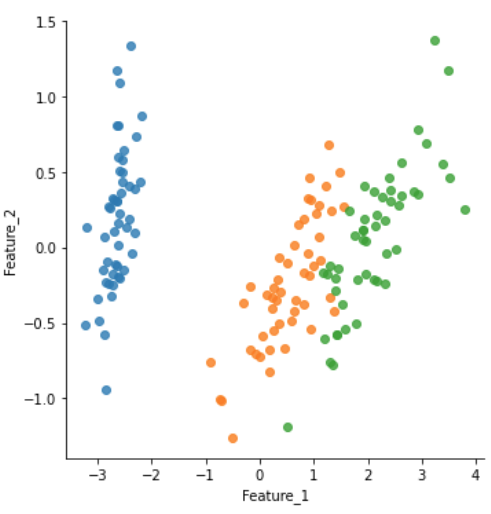
\includegraphics[width=8.0cm]{./pic/Clustering_Beispiel.png}
    \caption{Beispiel für Clustering}
    \label{fig:Clustering_Beispiel}
\end{figure}

Bei der ,,\textit{Dimensionality Reduction}'' versucht der Algorithmus das Datenset in seiner 
Dimensionalität, also in der Anzahl an Feldern, zu reduzieren. Es wird also die Frage gestellt, 
ob sich in einem bestehenden Datenset auch mit weniger Feldern Abhängigkeiten feststellen lassen. Dieser 
Schritt wird vor allem für Modelle benutzt, die sensibel gegenüber hoher Dimensionalitäten sind, 
sodass das Datenset vor dem Training in seiner Dimensionalität heruntergebrochen werden kann.

Im Rahmen des Projektes wurden hauptsächlich Klassifizierungs-Algorithmen genutzt, da ein Großteil der 
Datensets Labels zur Überprüfung hatte.\\
Um einen Vergleich zu ermöglichen, werden später trotzdem noch 
einzelne Ergebnisse von Clustering und Dimensionality Reduction betrachtet. Im Folgenden sollen die genutzten 
Modelle erklärt werden.
\newpage
\subsection{Random Forest Classifier}

\textit{Random Forest Classifier} RFC stellen eine Unterkategorie der ,,\textit{Decision Trees}'' dar. Decision Trees sind einfache
Anordnungen von bestimmten Fragen, die über das Datenset gestellt werden, um eine Klassifikation zu erreichen.

\begin{figure}[h]
    \centering
    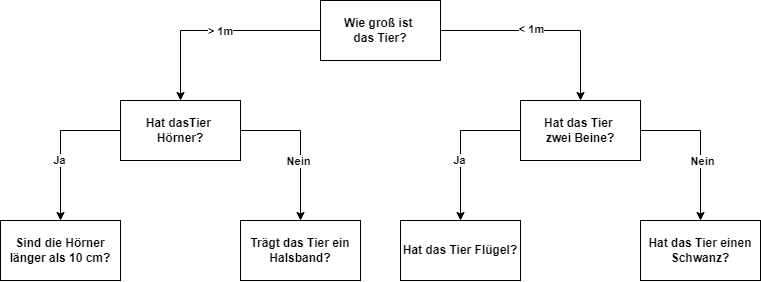
\includegraphics[width=10.0cm]{pic/DecisionTree.png}
    \caption{Beispiel eines Decision Trees}
    \label{fig:DT_Beispiel}
\end{figure}

Erstellt man ein ,,\textit{Ensemble}'' aus Decision Trees, die Erwartungen über einen zufällig gewählten 
Teil des Datensets treffen können, entsteht ein Random Forest. Der Teilname \textit{Random} bedeutet, dass
jeder Decision Tree des Ensenbles ein zufällig gewähltes Subset an Spalten des Datensets enthält.\\
Der Random Forest Classifier versucht, eine Menge einfacher Schätzfunktionen über einen komplexeren 
Sachverhalt ,,abstimmen'' zu lassen. Während sich in einem einzelnen Entscheidungsbaum Fehleinschätzungen 
entwickeln können, sinkt die Chance auf eine solche Fehleinschätzung, je mehr unabhängige 
Entscheidungsbäume man befragt. 

\subsection{Gradient Boosting Classifier}
Der \textit{Gradient Boosting Classifier} GBC ist eine Abwandlung eines RFC und  versucht, seine Erwartungen
aufgrund von Abweichungen eines Labels vom Durchschnitt dieses Labels zu treffen. \\
Versucht man beispielsweise aus dem Gewicht eines Tieres dessen Alter zu bestimmen, wird 
ein GBC als Ausgangswert den Durchschnitt aller Label-Werte, also dem Alter, berechnen. Danach werden die 
Abweichungen aller Label-Werte zu diesem Durchschnitt gebildet. Diese Abweichungen werden nun in Beziehung zu den 
anderen Spalten des Datensets gesetzt. 
\\\\
Beispielsweise könnte man so davon ausgehen, dass ausgewachsene Tiere von einem 
bestimmten Alter über dem Durchschnittsgewicht liegen. Genauso liegen besonders junge Tiere wahrscheinlich immer
einen ähnlichen Wert unter dem Durchschnittsgewicht. So wurde zwischen dem Label \textit{Gewicht} und der Spalte 
\textit{Alter} eine Beziehung hergestellt. In weiteren Iterationen orientiert sich der GBC immer an der Abweichung 
zum Durchschnittswert des vorherigen Baumes. So werden die getroffenen Erwartungen über mehrere Iterationen immer 
präziser.
\newpage
\subsection{Support Vector Classifier}
Der \textit{Support Vector Classifier} SVC versucht in einem Datenset anhand von bestimmten Cut-Off-Values klare Grenzen 
zwischen Werten zu finden, sodass man alle Messwerte ober- und unterhalb der Grenze eindeutig klassifizieren 
kann.

\begin{figure}[h]
    \centering
    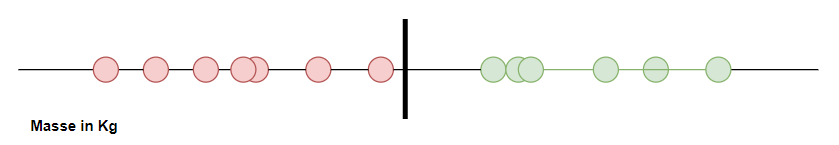
\includegraphics[width=10.0cm]{pic/SVC_1D.png}
    \caption{Beispiel eines Support Vector Classifiers}
    \label{fig:SVC_1D}
\end{figure}

In Abb. \ref{fig:SVC_1D} ist der SVC ein Punkt auf einer eindimensionalen Linie, auf der das Gewicht in kg von z.B. 
Tieren in ,,unter-'' und ,,übergewichtig'' unterteilt wird. Dieser Punkt ist Ergebnis aller Verhältnisse der einzelnen
Datenpunkte zueinander. Der SVC versucht sich dabei stets so zu positionieren, dass sein Abstand zu den beiden nächsten
grünen und roten punkten minimal wird. Die Position wird zusätzlich durch die Verteilung der Datenpunkte gewichtet.\\
Durch sog. ,,\textit{Kernel Funktionen}'' versucht der Algorithmus nun Beziehungen 
in höheren Dimensionen zu finden, wie z.B. $Masse^2$, $Masse^3$ usw. . Der SVC stellt dann in diesen Dimensionen 
eine Linie in einem zweidimensionalen oder eine Ebene in einem dreidimensionalen Koordinatensystem usw. dar.\\

\begin{figure}[h]
    \centering
    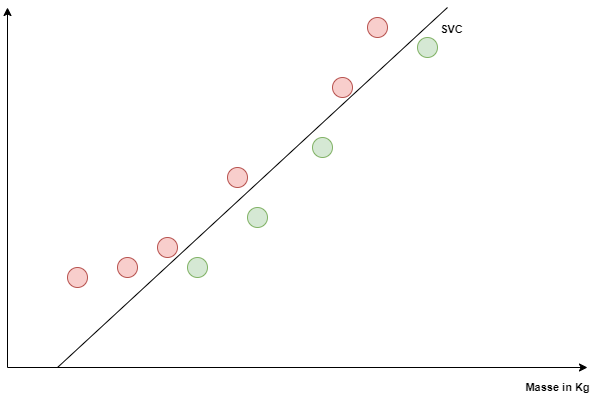
\includegraphics[width=10.0cm]{pic/SVC_2D.png}
    \caption{Beispiel eines Support Vector Classifiers in der zweiten Dimension}
    \label{fig:SVC_2D}
\end{figure}

Da der SVC die Verhältnisse aller Datenpunkte zueinander betrachtet, ist er sehr anfällig für Abweichungen in 
den Daten, was bei der Datenvorbereitung und der Auswertung beachtet werden muss.

\newpage
\subsection{Logistische Regression}

Die \textit{Logistische Regression} LR ordnet Daten anhand einer Wahrscheinlichkeit einem bestimmten Label  zu. Trotz des Teilnamens
,,Regression'' handelt es sich um einen Klassifizierungsalgorithmus. Der Name kommt daher, dass die berechnete Wahrscheinlichkeit
zu einem kontinuierlichen Label zwischen 0 und 1 führt, was durch die Form einer Sigmoid-Funktion ausgedrückt wird.
Der Algorithmus eignet sich wegen dieser Eigenschaft besonders für  das Klassifizierungsproblem der Projektarbeit, 
bei der ein Wahrheitswert, wie ,,Anwesenheit'' oder ,,Abwesenheit'' untersucht werden soll.\\
Nutzt man logistische Regression beispielsweise zur Abbildung einer Beziehung zwischen Gewicht von Tieren in Gramm 
zu einer Wahrscheinlichkeit für Übergewicht, könnte das entstehende Modell wie folgt aussehen.

\begin{figure}[h]
    \centering
    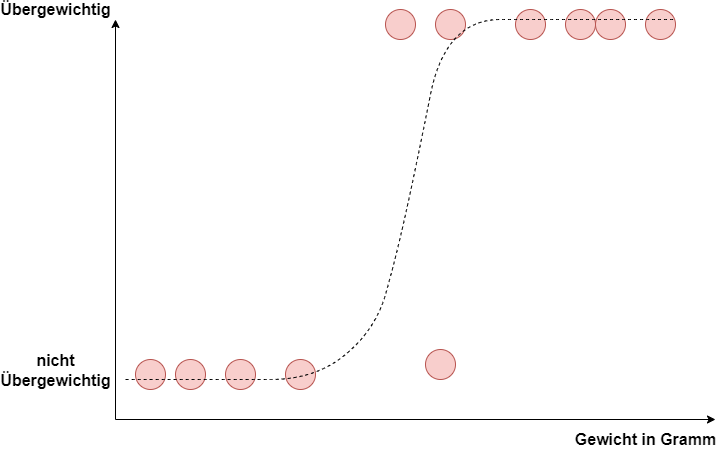
\includegraphics[width=10.0cm]{pic/logistic_regression.png}
    \caption{Beispiel logistischer Regression}
    \label{fig:LR}
\end{figure}

Die Sigmoid-Funktion wird grundsätzlich durch

\begin{align}
    p = \frac{1}{1 + e^{-(x-\mu)/s}}
\end{align}

beschrieben, wobei x der Eingabewert in Gramm darstellt und $\mu$ der Mittelpunkt der Kurve beschreibt, der sich aus dem 
Verhältnis von Eintrittswahrscheinlichkeit $p_1$ und Gegenwahrscheinlichkeit $p_0$ ergibt.

\begin{align}
    p(\mu) = 0.5 = \frac{p_1}{p_0}   
\end{align}

\newpage
Zusätzlich beschreibt s einen Skalierungsparameter, mit dem die Form der Kurve flacher oder steiler werden kann,
was angibt, wie eindeutig die eingegebenen Daten zugeordnet werden können. Wären im o.g. Beispiel also alle roten
Punkte jeweils links und rechts von der Mitte einsortiert, wäre die Sigmoid-Funktion in der Mitte sehr steil, da alle
Daten anhand des Mittelpunktes klar getrennt werden könnten.

\begin{figure}[h]
    \centering
    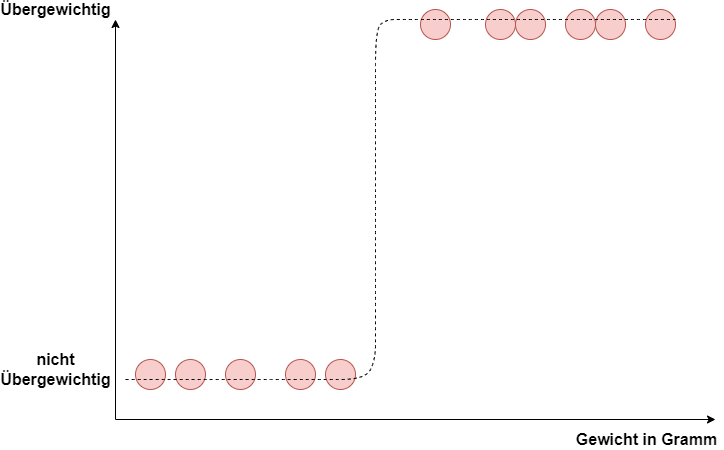
\includegraphics[width=10.0cm]{pic/logistic_regression_high s.png}
    \caption{Logistische Regression mit deutlicher Skalierung}
    \label{fig:LR_scal}
\end{figure}

Anhand der optimierten Sigmoid-Funktion können nun neue Daten klassifiziert werden, wobei die Wahrscheinlichkeit
bei $p < 0.5$ auf 0 und $p >= 0.5$ auf 1 gerundet wird.
\newpage
\subsection{K-Nearest-Neighbours Clustering}
Der \textit{K-Nearest-Neighbours}-Algorithmus KNN betrachtet den Abstand von einem gegebenen Punkt $p$ zu einer 
Menge an Punken in einem Datenset und ordnet ihn gemäß dieser Abstände einer bestimmten Kategorie zu. Die 
Zuordnung geschieht anhand der Kategorie der größten Menge zum nächsten Nachbarn.

\begin{figure}[h]
    \centering
    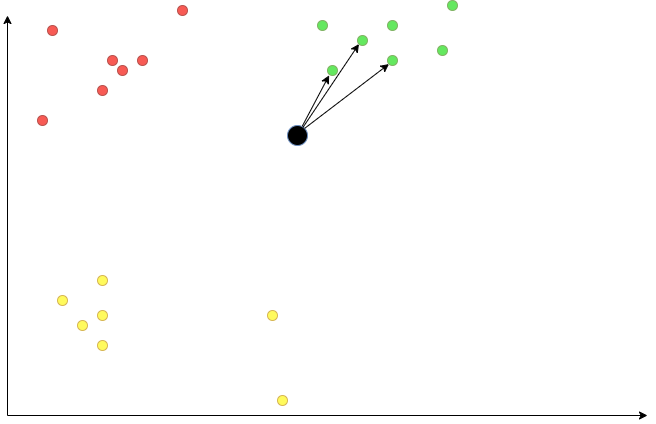
\includegraphics[width=12.0cm]{pic/KNN.png}
    \caption{Beispiel eines KNN}
    \label{fig:KNN}
\end{figure}

Im oben gezeigten Beispiel würde ein Punkt anhand seiner drei nächsten Nachbarn als ,,grün'' kategorisiert.
Die Anzahl der gewünschten Nachbarn, die zu untersuchen sind, ist frei wählbar.
Da die Abstandsberechnung über den \textit{Euklidischen Abstand} berechnet wird, funktioniert dieser 
Algorithmus auch in höheren Dimensionen, denn

\begin{align}
    d = \sqrt{(x2 - x1)^2 + (y2 - y1)^2 + (z2 - z1)^2 + ... + (n2 - n1)^2}
\end{align}

lässt sich für beliebig viele Dimensionen fortsetzen.

\newpage

\subsection{K-Means Clustering}
Der \textit{K-Means} Algorithmus legt eine bestimmte Anzahl von neuen Datenpunkten an eine zufällige Position des
Datensets.  Die herumliegenden Datenpunkte werden nun anhand ihrer Abstände diesen sog. \textit{Clustern} 
zugeordnet (in Abb. \ref{fig:KMeans1} als vertikale Linien dargestellt).\\
Die Abstände werden auch hier durch die Euklidische Abstandsformel berechnet.\\

\begin{figure}[h]
    \centering
    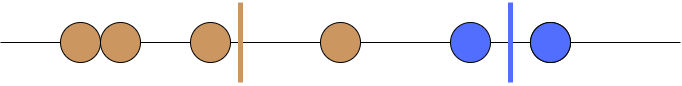
\includegraphics[width=12.0cm]{pic/KMeans_step1.png}
    \caption{Beispiel des K-Means Algorithmus}
    \label{fig:KMeans1}
\end{figure}

Da der Algorithmus die optimale Verteilung von Clustern nicht erkennen kann, wird die Position der Cluster 
gespeichert und neue Cluster an zufällige Positionen gelegt. Sind die durchschnittlichen Abstände der Datenpunkte
zu den neuen Clustern geringer als vorher, werden die gespeicherten Cluster nun in Richtung der neuen Cluster 
verschoben (Abb. \ref{fig:KMeans2}).\\

\begin{figure}[h]
    \centering
    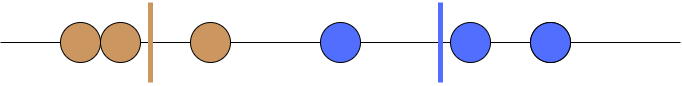
\includegraphics[width=12.0cm]{pic/KMeans_step2.png}
    \caption{Beispiel des K-Means Algorithmus}
    \label{fig:KMeans2}
\end{figure}

Die Anzahl an Schritten, die der Algorithmus durchläuft, kann vorgegeben werden. Allgemein sollte der Algorithmus
so lange neue Schritte machen, bis der Abstand der gespeicherten und neuen Cluster zueinander einen bestimmten
Minimalwert unterschreitet.

\newpage
\subsection{Neuronale Netzwerke}
Die Funktionsweise eines neuronalen Netzwerks ist direkt angelehnt an die Funktionsweise des menschlichen Gehirns.
Einzelne Knotenpunkte (Neuronen) werden mithilfe von gewichteten Verbindungen verknüpft, sodass das Netzwerk versucht 
Eingabewerte bestimmten Ausgabewerten zuzuordnen. Diese Zuordnung der Ein- und Ausgabewerte im Input- und Output-Layer 
geschieht nicht direkt, sondern durch ein oder mehrere \textit{Hidden Layer}, dessen Neuronenzahl üblicherweise über 
der Anzahl der Neuronen im Input Layer liegt. Die Anzahl der Neuronen im Output-Layer entspricht der Anzahl an Ergebnissen, 
die sich aus dem Input ergeben können. Im Beispiel der Anwesenheitsanalyse entspräche das also zwei Neuronen für 
An- und Abwesenheit.

\begin{figure}[h]
    \centering
    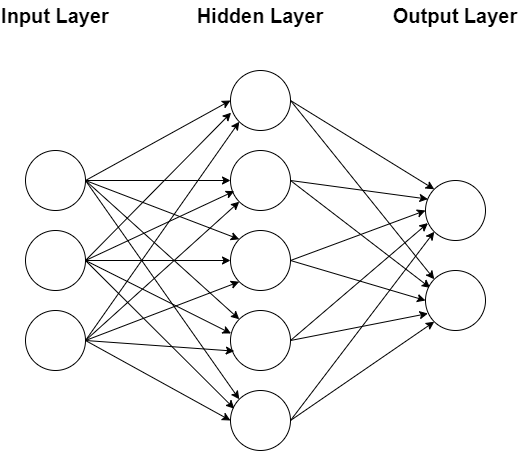
\includegraphics[width=10.0cm]{pic/NN.png}
    \caption{Beispiel eines neuronalen Netzwerks}
    \label{fig:NN}
\end{figure}

Liegt an einem Neuron eine Information an, wird diese als Eingabe einer Aktivierungsfunktion $\varphi$ genutzt, 
die mithilfe eines bestimmten Schwellwertes bestimmt, ob dieses Neuron aufgrund der Eingabe aktiviert wird. Über eine 
bestimmte Anzahl von Iterationen werden die Gewichtungen zwischen den einzelnen Neuronen stärker oder schwächer.


\subsection{Long Short Term Memory}
Das \textit{Long Short Term Memory} LSTM ist eine Abwandlung herkömmlicher neuronaler Netzwerke. Es handelt sich um ein
\textit{rekurrentes} neurales Netzwerk, was bedeutet, dass jedes Neuron seine Ausgabewerte auch wieder als Eingabewerte
nutzt. Der Begriff \textit{Memory} rührt daher, dass durch diese Rückkopplung eine Art Gedächtnis entsteht, durch 
die das Netzwerk bessere Rückschlüsse auf die Einordnung des aktuellen Input-Wertes ziehen kann.\\

\begin{figure}[h]
    \centering
    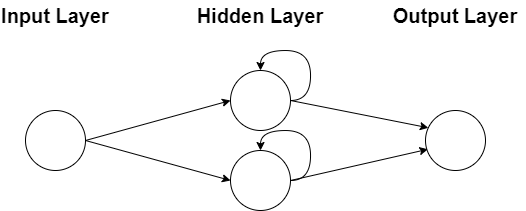
\includegraphics[width=10.0cm]{pic/RecurrentNN.png}
    \caption{Beispiel eines rekurrenten neuronalen Netzwerks}
    \label{fig:RecNN}
\end{figure}
\newpage
Bei einem LSTM verfügt jedes Neuron zusätzlich über einen Zell-Status $C_t$, welcher durch einen Input $x_t$ verändert werden kann.
Auf den Zell-Status nehmen \textit{Input-}, \textit{Forget-} und \textit{Output}-Gates Einfluss. Diese drei Gates
besitzen jeweils ein eigenes neuronales Netzwerk $\sigma$.\\\\
Das Input-Gate bestimmt, ob der Zell-Status anhand des anliegenden Inputs verändert werden darf.
Das Forget-Gate gibt an, ob der Status der Zelle zurückgesetzt und somit das ,,Gedächtnis'' der Zelle gelöscht wird. Es
stellt die zentrale Komponente des LSTMs dar.
Das Output-Gate regelt, ähnlich wie Aktivierungsfunktion normaler NNs, ob der anliegende Input zu einem Output 
der Zelle führt.

\begin{figure}[h]
    \centering
    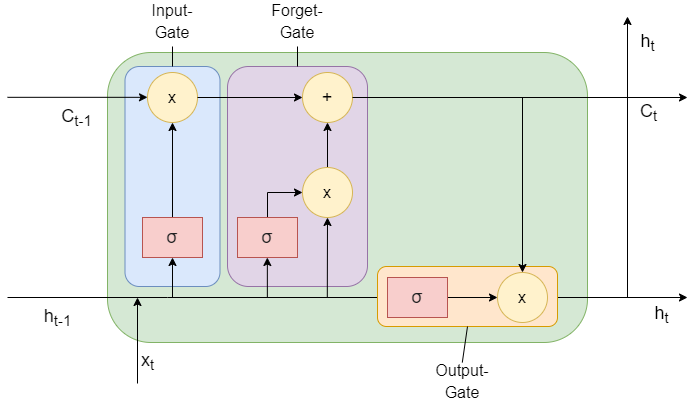
\includegraphics[width=12.0cm]{pic/LSTM-Cell.png}
    \caption{Vereinfachter Aufbau einer LSTM-Zelle}
    \label{fig:LSTM_Cell}
\end{figure}

Ein LSTM kann auf diese Weise eine Vielzahl vorangegangener Zeitschritte einbeziehen. Es verlässt sich so nicht 
direkt auf einen gegebenen Input, sondern auf einen langen Verlauf von bereits verarbeiteten Input-Werten. 
LSTMs sind deshalb besonders interessant für Probleme bei denen Beziehungen zwischen kontinuierlichen 
Datenwerten gebildet werden müssen.

\newpage
Man gehe man von einem LSTM aus, das über eine Liste an Namen verfügt und anhand eines Datensatzes gelernt
hat, zwei Namen mit der Beziehung ,,sah'' zu z.B. ,,Jonas sah Jakob.'' zu verknüpfen.\\
Das LSTM hat nun intern einen Status, der angibt, dass auf einen Namen mit hoher Wahrscheinlichkeit das Wort 
,,sah'' und mit niedriger Wahrscheinlichkeit ein zweiter Name folgt. 
Beginnt man nun einen neuen Satz mit ,,Jakob'', werden als mögliche nächste Worte ,,Jonas'', ,,Jakob'' und ,,sah''
ausgewählt. Bisher ähnelt dieser Verlauf einem normalen neuronalen Netzwerk. Beim LSTM
steht aber nun wegen des vorherigen Durchlaufs der Name ,,Jakob'' im Forget-Gate, sodass ,,Jakob'' aus der verfügbaren
Wortauswahl für das nächste Wort gelöscht wird.\\



\section{CO2 als Anwesenheitsindikator}\label{CO2}

%Der CO2-Gehalt der Raumluft ist als sehr guter Indikator für menschliche Präsenz anzusehen. Anders als andere 
%Umweltindikatoren wie Temperatur oder Luftfeuchtigkeit hat der CO2-Gehalt die Eigenschaft, dass es in 
%geschlossenen Räumen keine äußeren Einflussfaktoren für diesen Messwert gibt. In einem Büroraum kann der 
%Mensch als alleinige Quelle für CO2 angesehen werden.\\
Der Anteil von CO2 in frischer Atemluft beträgt zwischen 350 und 450 ppm. Es gibt in Deutschland und auch Europa 
keine grundsätzlich festgelegten Grenzwerte für akzeptable Raumluft, vielmehr raten Gesundheitsämter 
verschiedener Länder Grenzwerte zwischen 1200 und 1500 ppm einzuhalten. Ab der Obergrenze von 1500 ppm 
zeigen sich beim Menschen erste Müdigkeitserscheinungen, weshalb dieser Wert in der Literatur als maximaler 
Richtwert für Innenräume gilt.\\

\begin{figure}[h]
    \centering
    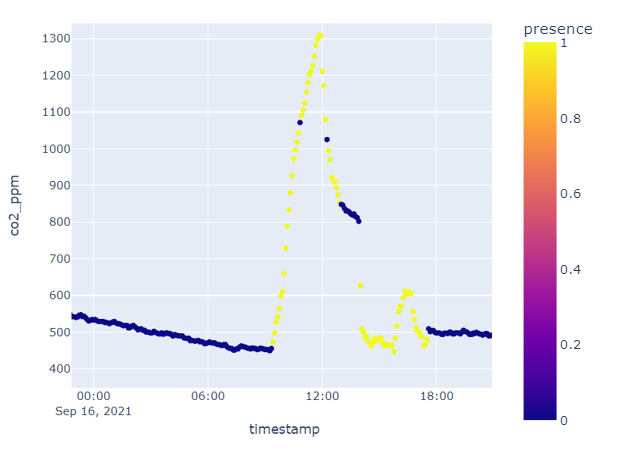
\includegraphics[width=0.7\textwidth]{pic/co2_singleDay.png}
    \caption{CO2-Gehalt der Raumluft über einen Tag}
    \label{fig:CO2_oneDay}
\end{figure}
 
Es ist zu erkennen, dass die CO2-Werte in einem normalen Büroraum innerhalb dieser empfohlenen Grenzen schwanken.
Abgesehen von einigen kleinen Pausen sind fast durchgehend Personen anwesend, die täglich etwa um 12:00 Uhr den 
Raum lüften.
Es ist auch klar zu erkennen, dass sich der CO2-Gehalt während der Abwesenheit von Personen durch die passive
Lüftung des Raumes (Tür-/Fensterspalten) langsam wieder gegen den Grundwert bewegt.

\newpage
\section{Luftfeuchtigkeit und Temperatur}
Auch wenn Luftfeuchtigkeit und Temperatur Indikatoren für menschliche Präsenz in einem Raum sein können, 
unterscheidet sich deren Aussagekraft von der des CO2-Gehaltes der Raumluft in einem wichtigen Faktor.\\ 
Sie werden beide stark von äußeren Umweltfaktoren wie dem aktuellen Wetter oder der Jahreszeit beeinflusst.
Beide Werte wurden zunächst in das Training aller Modelle miteinbezogen; es wird allerdings im folgenden 
Kapitel gezeigt, dass diese beiden Werte zusammen mit dem CO2-Wert wenig aussagefähig sind und 
deshalb später nicht weiter genutzt werden.  

\section{Sensordaten}
Wie bereits beschrieben, wurden die Sensordaten in mehreren Räumen der FH Aachen kontinuierlich 
gesammelt. Durch das Filtern nach den einzelnen Räumen kann für jeden Raum ein Datenset nach folgender Struktur
erzeugt werden:\\

\begin{table}[ht]
    \caption{Sensordaten}
    \centering
    \begin{tabular}{|p{4.5cm}||p{3cm}|p{5.5cm}|}
        \hline
        \multicolumn{3}{|c|}{Sensordaten} \\
        \hline
        Name&Format &Beschreibung\\
        \hline
        timestamp&timestamp&Zeitpunkt der Messung\\
        co2\_ppm&integer&CO2-Wert\\
        temperature\_celsius&float&Temperatur in Grad Celsius\\
        relative\_humidity\_percent&float&Luftfeuchtigkeit\\
        presence&boolean&Aktivität Bewegungssensor\\
        \hline
    \end{tabular}             
\end{table}

\newpage
\chapter{Technische Umsetzung}

\section{Datenbeschaffung und -Vorbereitung}
Die Daten wurden lokal auf einem der FH-Server in Form eines \textit{Hadoop Distributed File System} (HDFS) 
gespeichert. Mithilfe von Apache Drill waren die Daten jederzeit durch einfache SQL-Abfragen abrufbar. 
Die Daten wurden so während der gesamten Dauer des Projektes immer aktuell gehalten, damit alle Erkenntnisse 
jeweils auf der aktuellsten Datenlage basieren.
\\\\
Die Datenvorbereitung (Pre-Processing) ist einer der wichtigsten Schritte bei der Anwendung von Machine 
Learning. Dadurch besteht die Möglichkeit, beim Training des Modells durch Bearbeitung bestehender Spalten
oder Hinzufügen zusätzlicher Spalten im Datenset Schwerpunkte zu setzen, die es den Algorithmen beim Training
zum einen erleichtern, ihre Erwartungen zu präzisieren, zum anderen aber auch deren Leistung bei der Verarbeitung
bestimmter Spalten zu steigern.
\subsection{Gruppierung}
Die Sensordaten wurden alle sechs Sekunden erfasst. Da sich weder CO2-Gehalt noch Feuchtigkeits- oder 
Temperaturwerte der Raumluft so schnell nicht verändern, wurden die Daten direkt beim Drill per SQL zu 
zwei-Minuten-Intervallen zusammengefasst. Dabei werden über alle Spalten hinweg Durchschnittswerte gebildet, 
die dann zu einem Datensatz zusammengefasst werden. 
Dies steigert die Leistung aller Algorithmen erheblich, weil sich dadurch die Zahl der 
Datensätze stark verringert. Da sich, wie oben erwähnt, der CO2-Gehalt der Raumluft in einem 
Intervall von zwei Minuten kaum merklich verändert, verringert sich die Genauigkeit des gesamten Datensets
dadurch nicht maßgeblich.
\subsection{Zyklische Codierung}
Zyklische Codierung wird immer dort verwendet, wo Daten sich in wiederholenden Schemata bewegen. Diese 
Schemata, wie z.B. die Zahlenumbrüche bei einer Uhrzeit, sind für Algorithmen nicht direkt ersichtlich und 
sind zudem für Computer nicht leicht zu verarbeiten. Durch eine Encodierung in 
Sinus- und Cosinus-Werte können diese Zusammenhänge vereinfacht werden.\\
Hierzu wurde der Timestamp zuerst in Sekunden übersetzt, sodass sich ein bestimmter Zeitpunkt eines Tages 
immer zwischen 0 und 86399 Sekunden bewegt.
Aus diesem Wert wurden dann zwei neue Datenspalten ,,\textit{hour\_sin}'' und ,,\textit{hour\_cos}'' 
in das Datenset eingefügt, welche sich aus 

\begin{align}
    hour\_sin = sin(2 * \pi * x / x_{max}) \\ 
    hour\_cos = cos(2 * \pi * x / x_{max})
\end{align} 

ergeben. So kann jede Tageszeit einer eindeutigen Kombination aus Sinus- und Cosinus-Werten zwischen 
$0$ und $1$ zugeordnet werden.

\subsection{Deltas und Shift-Werte}
Desweiteren wurden von den Spalten ,,\textit{co2\_ppm}'', ,,\textit{temperature\_celsius}'' und \break 
,,\textit{relative\_humidity\_percent}'', die tatsächlich Rückschlüsse auf die Präsenz zulassen, \break 
zusätzliche Delta- und Shift-Spalten angelegt.\\\\
Ein Shift-Wert bedeutet lediglich, dass  in einer Zeile $x_n$ des Datensets 
zusätzlich, neben den aktuellen Werten, auch Werte von $k$ Zeilen zuvor, also $x_{n-k}$ stehen. So haben 
alle Algorithmen direkten Zugriff auf Vergangenheitswerte der ausgewählten Spalten.\\\\
Delta-Spalten stellen, dem Namen nach, Deltas zu vorherigen Werten dar:

\begin{align}
    \Delta x_k = x_n - x_{n-k}    
\end{align}

Die Erwartung ist hier, dass die Änderung der CO2-, Temperatur- und 
Luftfeuchtigkeitswerte ein wichtigerer Indikator sein könnte, als die tatsächlichen Werte. In einem schlecht 
klimatisierten Raum könnten Grundwerte von z.B. CO2 höher sein, als in Räumen, in denen regelmäßig gelüftet wird.
Unabhängig dieser Grundwerte könnte man bei einem starken Anstieg wesentlich einfacher menschliche Präsenz erkennen, 
ohne dass zunächst die vorangegangenen Werte überprüft werden müssen.
Durch die hinzufügten 
Deltas werden diese Grundwerte ignoriert und Rückschlüsse auf die aktuelle Präsenz sind besser möglich.\\
Im Zuge der Projektarbeit wurden verschiedene Kombinationsmöglichkeiten von Delta- und Shiftwerten mit 
Zeitschritten zwischen zwei Minuten und einer Stunde mit Hinblick auf Verbesserungen der Modell-Genauigkeiten 
getestet.

\subsection{Outlier Detection}
Wie bereits erwähnt, spielen Datenausreißer für die Ergebnisse mancher Algorithmen eine große Rolle. Überall 
wo z.B. aus einer Reihe von Datenwerten Durchschnittswerte berechnet werden, würden Ausreißer in den Daten das 
Ergebnis verfälschen und die Aussagekraft des Algorithmus deutlich senken.
Um diese Ausreißer vor dem Training der Modelle zu beseitigen, wurde das Verfahren des 
\textit{Interquartilabstands} (IQR nach der englischen Bezeichnung \textit{Interquartile Range}) gewählt.\\
Der IQR gibt die Intervallgröße an, die ein Wert vom Median einer Datenreihe abweichen darf. Bei einer 
der Größe nach sortierten Datenreihe $x = (x_0,x_1,...,x_n)$ bestimmt man die Mediane der unteren und oberen 
Hälfe des Datensets $Q_1$ und $Q_2$. Der IQR ergibt sich nun aus 
\begin{align}
    IQR = Q_2 - Q_1
\end{align}
Mit diesm Wert können jetzt die erlaubten Ober- und Untergrenzen 
des Datensets mit 
\begin{align}
    Limit_{upper} = Q_2 + 1.5 * IQR \\
    Limit_{lower} = Q_1 - 1.5 * IQR
\end{align} 
bestimmt werden. Alle Werte die außerhalb dieser Grenzen liegen, können als Ausreißer betrachtet werden.\\
Ausreißer zu entfernen, ist hier wichtig, da die Sensoren Messfehler erzeugen können und einige Modelle dadurch,
wie bereits beschrieben, stark beeinflusst werden können.

\section{Validierung}
\sloppy
Über das Projekt hinweg wurden verschiedene Validierungsmethoden verwendet. Grundsätzlich unterteilt man das 
Datenset in ein Trainings- und Testset mit einem Verhältnis von etwa 80-20. Das bedeutet, dass das Modell mit
80 Prozent der Daten trainiert wird, wobei die anderen 20 Prozent zurückgehalten werden, um daraufhin das 
fertig trainierte Modell daran zu testen. Aus dem Ergebnis dieses Tests ergeben sich verschiedene Werte, die  
die allgemeine Genauigkeit des Modells repräsentieren, d.h. wie verlässlich das Modell die An- und Abwesenheit 
des Testsets selbst berechnen kann, wenn man ihm den tatsächlichen Wert vorenthält.\\
Allgemeine Basis für die errechneten Genauigkeiten bildet die sog. \textit{Confusion Matrix}.

\begin{figure}[h]
    \centering
    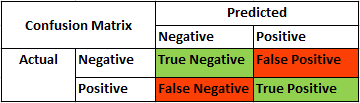
\includegraphics[width=0.6\textwidth]{pic/confusion_matrix_ex.png}
    \caption{Beispiel einer Confusion Matrix}
    \label{fig:CV}
\end{figure}

Diese zeigt, inwiefern die Genauigkeit des Modells neben tatsächlich richtig erkannten Werten zusätzlich
von false negatives und false positives beeinflusst wird.\\
\newpage
Die \textit{Accuracy Score} ist eine einfache Methode zur Bestimmung der Modellqualität und berechnet sich 
aus der Summe der richtigen Ergebnisse geteilt durch die Summe aller Ergebnisse.

\begin{center}
    $AccuracyScore = \dfrac{TP + TN}{TP + TN + FP + FN}$    
\end{center}
Die \textit{Recall Score} beschreibt die Genauigkeit bezogen auf alle erkannten positiven Ergebniswerte. 
%Dabei ist wichtig, dass wenn ein Algorithmus beispielsweise Anwesenheit zu erkennen versucht auch ein
%false negative als Treffer gewertet wird.
\begin{center}
    $RecallScore = \dfrac{TP}{TP + FN}$    
\end{center}

Die \textit{Precision Score} gibt die allgemeine Menge an positiven Werten an, die hätten erkannt werden müssen.
\begin{center}
    $PrecisionScore = \dfrac{TP}{TP + FP}$    
\end{center}

Die \textit{F1-Score} ist der Durchschnittswert aus Recall- und Precision-Score und liefert im Allgemeinen eine 
gute Auskunft über die Qualität eines Modells.\\

\begin{center}
    $F1\_Score = \dfrac{2}{\dfrac{1}{PrecisionScore} + \dfrac{1}{RecallScore}} = \dfrac{2 \cdot (PrecisionScore \cdot RecallScore)}{PrecisionScore + RecallScore}$    
\end{center}

\vspace{0.75cm}
In diesem Anwendungsfall ist es durchaus wichtig, Werte zur Anwesenheit von Personen genauer zu betrachten als 
Werte zur Abwesenheit, da die tägliche Arbeitszeit nur etwa ein Drittel eines ganzen Tages ausmacht. 
Da von 24 Stunden ca. 16 Stunden Werte zur Abwesenheit und nur etwa 8 Stunden Werte zur Anwesenheit enthalten, 
ist das Datenset also mit einem Verhältnis von etwa 1/3 in Richtung der Abwesenheit unausgeglichen. 
Dies lässt die Erwartung zu, dass das trainierte Modell wesentlich besser darin sein wird, Abwesenheit von Personen
zu erkennen, als Anwesenheit.\\
Hierzu wurde bei der Auswertung der Ergebnisse immer auch der \textit{Classification Report} hinzugezogen,
aus dem ersichtlich ist, wie genau das Modell beide möglichen Labelwerte berrechnen konnte.
\newpage
Desweiteren war es entscheidend zu erkennen, dass das Datenset über mehrere Monate hinweg nicht perfekt uniform 
ist, da in bestimmten Monaten verhältnismäßig viele Urlaubstage (z.B. Weihnachten/Silvester) vorkommen und es damit 
zu einer Häufung an Abwesenheitswerten kommt.
Wenn die Daten nun im o.g. Verhältnis aufgeteilt werden und dann viele Daten des Testsets in solchen Monaten 
liegen, könnte es beim Ergebnis zu Verzerrungen kommen.\\
Hierfür wurde eine \textit{Kreuzvalidierung} (engl. Cross Validation CV) implementiert. Bei einer CV wird das 
Datenset immer noch im gleichen Verhältnis aufgeteilt, allerdings mehrmals, sodass die Trainings- und Testsets 
jedes Mal aus jeweils anderen Daten bestehen.

\begin{figure}[h]
    \centering
    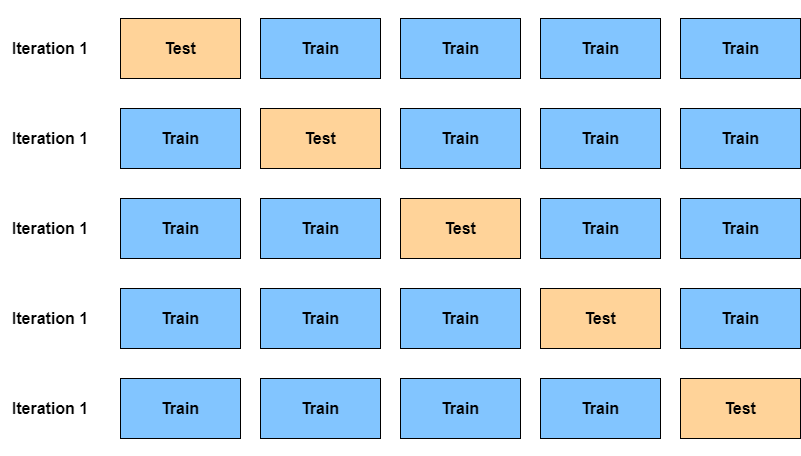
\includegraphics[width=0.7\textwidth]{pic/cv_new.png}
    \caption{Beispiel einer Kreuzvalidierung}
    \label{fig:CV}
\end{figure}

Errechnet man nun die Durchschnittsgenauigkeit aller Iterationen der CV, ergibt sich eine Gesamtgenauigkeit, 
die das Model besser repräsentiert, weil es mit einer größeren Anzahl von verschiedenen Daten trainiert und 
getestet wurde.
\\\\
Da es für manche Räume keine Datensätze mit Labelwerten gab, musste die Validierung dieser Datensätze 
augenscheinlich erfolgen. Hierfür wurde in ein Datenset eine Labelspalte eingefügt, die dann vom trainierten
Modell selbst gefüllt werden sollte. Das Ergebnis musste schließlich als Graph gezeichnet und per Hand validiert 
werden. Da sich das Ergebnis der Berechnung in diesem Anwendungsfall, wie oben gezeigt, sehr übersichtlich als 
Graph darstellen lässt, war diese Methode der Validierung zwar nicht perfekt, lieferte aber trotzdem einen 
ausreichenden Eindruck über die Qualität des trainierten Modells.


\subsection{Over- und Underfitting}
Over- und Underfitting sind Probleme, die bei allen Machine Learning Algorithmen auftreten können und bezeichnen 
im Allgemeinen einen falschen Umgang mit dem Datenset.
\textit{Overfitting} bedeutet, dass das Modell mit zu vielen, sich zu stark ähnelnden, Daten trainiert wurde, 
wodurch es in der Lage ist, nur neue Daten richtig zu kategorisieren, die dem Trainingsset besonders ähnlich sind.
Overfitting kann während einer Kreuzvalidierung oder der Validierung anhand eines anderen Datensets als dem 
Trainingsset erkannt werden.\\
Um Overfitting zu verhindern, kann das Datenset vereinfacht werden, um so die Beziehungen zwischen den
für die Erwartungsberechnung relevanten Spalten zu stärken.\\\\
\textit{Underfitting} bedeutet dagegen, dass es das Modell nicht geschafft hat, zwischen den gegebenen Daten
Beziehungen herzustellen, sodass das Modell unbekannte Daten richtig kategorisieren kann. Hier reicht es 
normalerweise aus, dem Modell mehr Daten zur Verfügung zu stellen und in der Datenvorbereitung Felder 
einzufügen, die dem Modell bestimmte Beziehungen zwischen Datenfeldern hervorheben sollen. 

\subsection{Parameter Tuning}
\textit{Parameter Tuning} beschreibt einen Schritt der Modell-Optimierung, der normalerweise stattfindet, 
nachdem ein funktionierendes Modell erstellt wurde, das mit bereits verarbeiteten Daten gute Ergebnisse liefert.
Jedes Modell besitzt Parameter, die bei der Erstellung festgesetzt werden. Diese Parameter haben 
großen Einfluss auf den Trainingsprozess, weshalb es sich anbietet, die Genauigkeiten mehrerer Modelle 
mit verschiedenen Parameter-Kombinationen zu testen.\\
Das im Scikit-Learn enthaltene \textit{GridSearchCV}-Modul
bietet die Möglichkeit, einem Modell eine Vielzahl von verschiedenen Parameter-Optionen zu übergeben. Mit diesen 
werden dann automatisch Modelle trainiert und per Kreuzvalidierung verglichen. Am Ende liefert das Modul 
die Parameter-Kombination, mit der das beste Ergebnis erzielt wurde.\\

\begin{figure}[h]
    \centering
    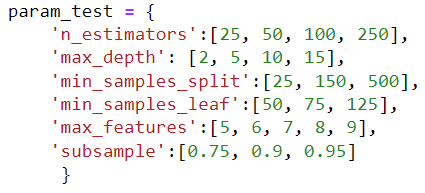
\includegraphics[width=0.6\textwidth]{pic/param_test.png}
    \caption{Beispiel einer Sammlung von Parameter-Optionen}
    \label{fig:Param_Test}
\end{figure}

Im obenstehenden Beispiel kann man erkennen, dass für bestimmte Parameter (rot) eine Sammlung an erlaubten 
Werten (grün) übergeben wird. Alle Kombinationen aus diesen Parameter-Optionen werden dann vom 
GridSearchCV-Modul ausgewertet.\\
Die Verbesserungen gegenüber Standard-Parametern bewegen sich normalerweise im niedrigen einstelligen 
Prozent-Bereich.
%% Zwei Abbildungen, die zusammen gehören

%\begin{figure}
%        \centering
%        \begin{minipage}[c]{0.45\textwidth}
%                \includegraphics[height=6.5cm]{pic/dateiname1.png}
%        \end{minipage}
%        \begin{minipage}[c]{0.45\textwidth}
%                \includegraphics[height=6.5cm]{pic/dateiname2.png}
%        \end{minipage}
%        \caption{Zwei Abbildungen}\label{fig:zwei_abb}
%\end{figure}

\clearpage
\chapter{\textbf{Anwendung und Ergebnisse}}\label{kap5}
%\addtocontents{toc}{\vspace{0.8cm}}

\section{Feature Vektor}
Der Feature Vektor FV beschreibt das Ergebnis des Datensets nach der Vorverarbeitung.
Die benutzten Felder werden bei jedem Anwendungsfall zunächst vom Programmierer selbst gewählt.
Durch die o.g. Schritte ergibt sich eine Vielzahl an möglichen zusätzlichen Features,
um die das Datenset erweitert werden kann. Es muss also zunächst ermittelt werden, welche dieser möglichen
Features wirklich aussagekräftig sind, um den FV nicht unnötig zu überladen. \\
Einige Algorithmen geben nach dem Training 
Auskunft darüber, in welchem Maß ein Feature in die Berechnung des Labels einfließt. Somit wurden zur Wahl eines
FVs, der nach dem Training mit einem Modell eine möglichst hohe Genauigkeit liefert, verschiedene Kombinationen 
von möglichen Feldern durch Verknüpfung von Temperatur, Luftfeuchtigkeit, CO2 mit jeweiligen Delta- und Shiftwerten 
vorgenommen. Anschließend werden die Modellgenauigkeiten einzelner FVs miteinander verglichen.

Ziel war es, mit einem möglichst kleinen Vektor eine möglichst hohe Genauigkeit zu erreichen, da bei den meisten Algorithmen eine 
direkte Abhängigkeit zwischen Dauer der Berechnung und Dimensionalität des FV besteht. \\\\ 

In diesem Fall wurden die Feature Importances eines Random Forest genutzt, um Auskunft darüber zu erhalten, wie 
relevant bestimmte Felder für die Erwartungsberechnung sind. Diese werden errechnet, indem geprüft wird, wie viele
Datensätze des Sets bestimmte Knoten des Baumes erreichen. Wenn ein beliebiger Decision Tree eine große Menge
des Datensets allein über seinen rechten Teilbaum klassifizieren kann, werden die darin enthaltenen Knoten schwerer
gewichtet, da sie in einem höheren Maß in die endgültige Entscheidung einfließen.\\\\

Diese Eigenschaft wurde zur Ermittlung des FVs genutzt, indem verschiedene Modelle mit einem FV-Kandidaten trainiert
wurden und anschließend sowohl die Genauigkeiten, als auch die Feature Importances gegenübergestellt wurden.
Features mit geringer Relevanz wurden entfernt und die Modellgenauigkeiten erneut geprüft, um so über mehrere 
Iterationen hinweg einen FV zu finden, dessen Felder möglichst hohe Aussagekraft besitzen, während die Anzahl 
nötiger Felder möglichst gering ist.\\\\

Hierzu wurden die Sensordaten zunächst um Delta- und Shiftwerte erweitert, um den Modellen die Möglichkeit zu geben
die aktuellen Werte den vorangegangenen Messungen gegenüberzustellen. Mit diesem FV wurde dann ein Random Forest
trainiert und dessen Feature Importances ausgewertet.

\newpage
\begin{figure}[h]
    \centering
    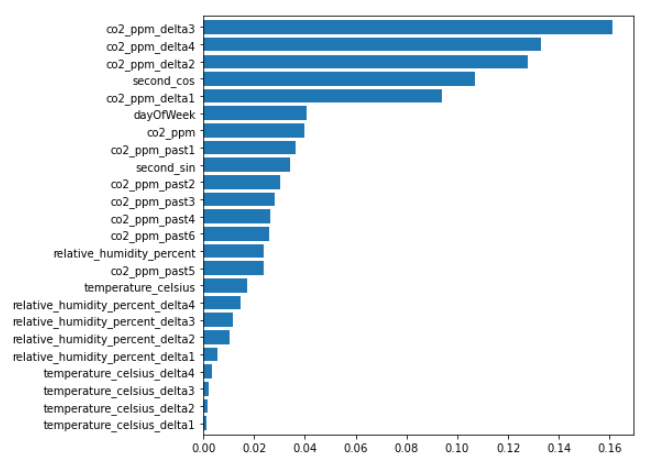
\includegraphics[width=1.0\textwidth]{pic/feature_importances.png}
    \caption{Feature Importances eines Random Forest}
    \label{fig:FI}
\end{figure}

Wie bereits im vorherigen Kapitel angedeutet, sieht man in Abb. \ref{fig:FI}, dass die Temperatur- und 
Luftfeuchtigkeitswerte für die Errechnung der Labels kaum zu Rate gezogen werden. 
Weder Grund- noch Deltawerte weisen eine hohe Relevanz für das Modell auf.\\
Es ist anzunehmen, dass Temperatur und Luftfeuchtigkeit an sich durchaus nützlich für solche Betrachtungen sein
können, allerdings werden sie durch die CO2-Werte in ihrer Relevanz übertroffen, da CO2 im Kontext menschlicher
Präsenz in Innenräumen eine deutlich höhere Aussagekraft besitzt.\\
%Zusätzlich weisen die Grundwerte Temperatur und Luftfeuchtigkeit über größere Zeiträume wetterbedingt starke 
%Schwankungen auf. Diese Schwankungen
%müssten von einem Modell zunächst von menschlicher Präsenz getrennt werden, da ein Temperaturanstieg nicht unbedingt
%Schlüsse auf Präsenz zulässt.\\
Die CO2-Werte sind für das Modell einfacher zu klassifizieren. Die Messwerte
eines CO2-Sensors erweisen sich als unabhängig von äußeren Einflüssen wie Jahreszeiten oder dem aktuellen Wetter 
und sind deshalb, wie in Abb. \ref{fig:FI} gezeigt, entscheidender Faktor bei der Berechnung.
\newpage
Nach anschließender Exkludierung von Temperatur und Luftfeuchtigkeit wurden neue Deltas und Shifts für die 
CO2-Werte eingefügt und die Feature Importances erneut betrachtet. 

\begin{figure}[h]
    \centering
    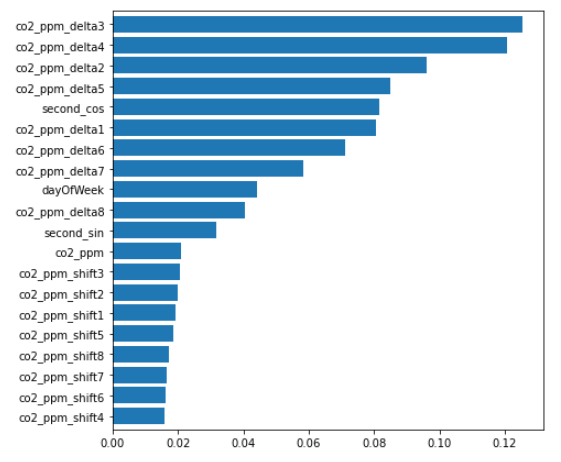
\includegraphics[width=0.9\textwidth]{pic/feature_importances_better.png}
    \caption{Feature Importances eines Random Forest}
    \label{fig:FIB}
\end{figure}

Es ist in Abb. \ref{fig:FIB} zu erkennen, dass die CO2-Shift-Werte ebenfalls nicht maßgeblich in die Berechnung einfließen. Diese weisen
allerdings noch deutlich höhere Feature Importances auf, als die Temperatur- und Luftfeuchtigkeitswerte.\\
Der Graph bestätigt die Annahme, dass beim CO2 die Deltawerte deutlich ausschlaggebender sind, als die 
tatsächliche Messung zu einem bestimmten Moment. \\

\newpage
Wenn diese Werte nur in solch geringem Maß zur Berechnung beitragen, muss ebenfalls die Schlussfolgerung daraus, 
dass die Genauigkeit auch ohne diese Werte innerhalb einer gewissen Toleranz konstant bleibt, überprüft werden.

Im Folgenden werden beispielhaft vier verschiedene Feature Vektoren beschrieben, aus denen der Vektor, der im 
weiteren Verlauf des Projektes benutzt werden sollte, abgeleitet wurde.
\begin{center}
    \begin{table}[h]
        \centering
        \caption{Vergleich Feature Vektoren}
        \begin{tabular}{ |c||c| } 
        \hline
        Feature Vektor & Beschreibung \\ 
        \hline\hline
        FV1 & CO2, Temperatur und Luftfeuchtigkeit mit Shift-Werten\\ 
        FV2 & CO2, Temperatur und Luftfeuchtigkeit ohne Shift-Werte \\ 
        FV3 & Nur CO2 mit Shift-Werten\\ 
        FV4 & Nur CO2 ohne Shift-Werte \\
        \hline
        \end{tabular}
    \end{table}
\end{center}

%\newpage
Mit diesen vier Vektoren wurden nun verschiedene Modelle trainiert und deren Genauigkeiten gegenübergestellt.

\begin{figure}[h]
    \centering
    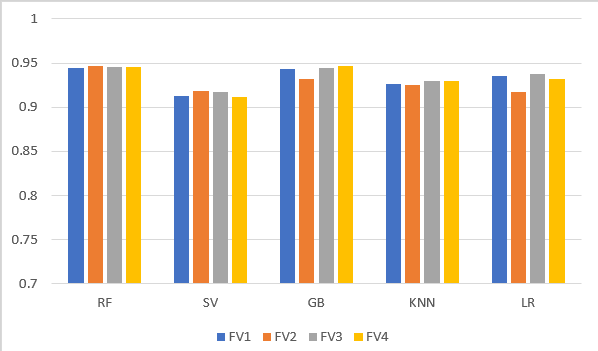
\includegraphics[width=0.8\textwidth]{pic/FV_comp.png}
    \caption{Vergleich der Genauigkeiten}
    \label{fig:FV_comp}
\end{figure}

Wie deutlich sichtbar ist, sind die Genauigkeiten fast identisch. Diese Gegenüberstellung wurde über das Projekt
hinweg mehrfach wiederholt und ergab immer ähnliche Unterschiede.\\
Dies war Anlass, sowohl die Temperatur- und Luftfeuchtigkeitswerte, als auch die Shift-Werte der CO2-Messungen 
nicht weiter zu betrachten, um den FV für Modelle mit hoher Empfindlichkeit gegenüber der Dimensionalität zu 
optimieren.

\newpage
Aus diesen Betrachtungen ergab sich folgender FV, der für den weiteren Verlauf des Projektes genutzt wurde:\\

\begin{center}
    \begin{table}[h]
        \centering
        \caption{Feature Vektor}
        \begin{tabular}{ |c||c| } 
        \hline
        Feld & Beschreibung \\ 
        \hline\hline
        second\_sin & timestamp-Sinusanteil\\
        second\_cos & timestamp-Cosinusanteil\\
        day\_of\_week & Wochentag der Messung\\
        co2\_ppm & CO2-Wert\\ 
        co2\_ppm\_delta1 & Delta zum CO2-Wert vor 2 Minuten\\ 
        co2\_ppm\_delta2 & Delta zum CO2-Wert vor 4 Minuten\\ 
        co2\_ppm\_delta3 & Delta zum CO2-Wert vor 6 Minuten\\ 
        co2\_ppm\_delta4 & Delta zum CO2-Wert vor 8 Minuten\\ 
        co2\_ppm\_delta5 & Delta zum CO2-Wert vor 10 Minuten\\ 
        co2\_ppm\_delta6 & Delta zum CO2-Wert vor 12 Minuten\\ 
        co2\_ppm\_delta7 & Delta zum CO2-Wert vor 14 Minuten\\ 
        co2\_ppm\_delta8 & Delta zum CO2-Wert vor 16 Minuten\\ 
        \hline
        \end{tabular}
    \end{table}
\end{center}

\newpage

\section{Ergebnisse}
Da nicht alle Algorithmen auf die gleiche Weise evaluiert und grafisch dargestellt werden können, sollen 
die Ergebnisse zu 
\begin{itemize}
    \item Decision Tree Modellen
    \item Neuronalen Netzwerken
    \item Clustering Modellen
\end{itemize}
einzeln betrachtet werden.

\subsection{Decision Tree Modelle}
Die ausgewählten Algorithmen konnten mit dem ausgewählten FV bei der Erwartungsberechnung über das gesamte 
Datenset eine Genauigkeit von etwa 94\% erreichen. Eine \textit{Confusion Matrix}, welche die errechneten 
Werte den tatsächlichen Labelwerten gegenüberstellt, zeigt, dass im hier benutzten Beispiel ein Random Forest Classifier 
selbst bei der starken Unausgeglichenheit des Datensets ähnlich viele Fehler bei sowohl An- als auch Abwesenheit 
von Personen macht.

\begin{figure}[h]
    \centering
    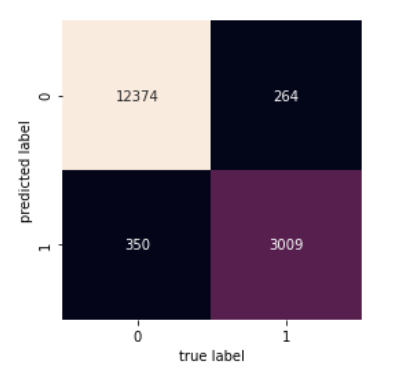
\includegraphics[width=0.5\textwidth]{pic/confusion_matrix.png}
    \caption{Confusion Matrix eines RFC}
    \label{fig:ConMatrix}
\end{figure}

In den Feldern oben links und unten rechts ist jeweils zu sehen, wann das Modell eine richtige Erwartung 
für jeweils Ab- und Anwesenheit errechnet hat, während die Felder oben rechts und unten links jeweils die 
Menge falscher Erwartungen für beide Werte zeigen.\\\\

\newpage
Ebenfalls aufschlussreich, ist die grafische Gegenüberstellung der erwarteten Labelwerte mit den tatsächlichen Labelwerten
indem man das ursprüngliche Datenset mit \textit{timestamp} und \textit{CO2-Wert} zeichnet. Dabei markiert geld die Anwesenheit
und blau die Abwesenheit von Personen.

\begin{figure}[h]
    \centering
    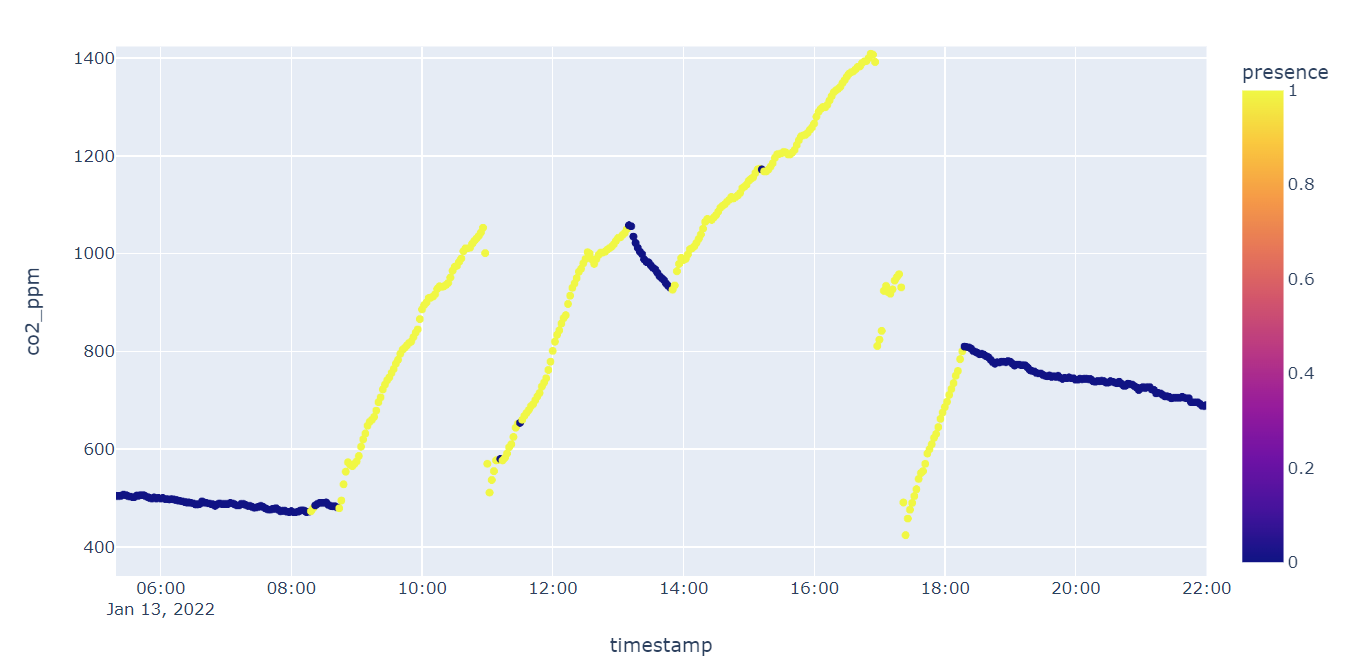
\includegraphics[width=0.9\textwidth]{pic/nov23_actual.png}
    \caption{Messwerte des 13. Januar}
    \label{fig:nov23}
\end{figure}

\ref{fig:nov23} zeigt den Verlauf der CO2-Messungen über einen Arbeitstag. Die blaue und gelbe Einfärbung stellt
die Messung des Infrarotsensors dar.\\ 
Ersetzt man aus dieser Datenreihe die tatsächlichen Messwerte des Infrarotsensors durch die errechneten 
Anwesenheitswerte des Modells, zeigt sich die hohe Genauigkeit in \ref{fig:nov23_pred} durch die neue Einfärbung 
der Datenreihe deutlich. 
Bis auf einige kleine Fehler trifft das Modell eine sehr präzise Aussage über die aktuelle Anwesenheit.

\begin{figure}[h]
    \centering
    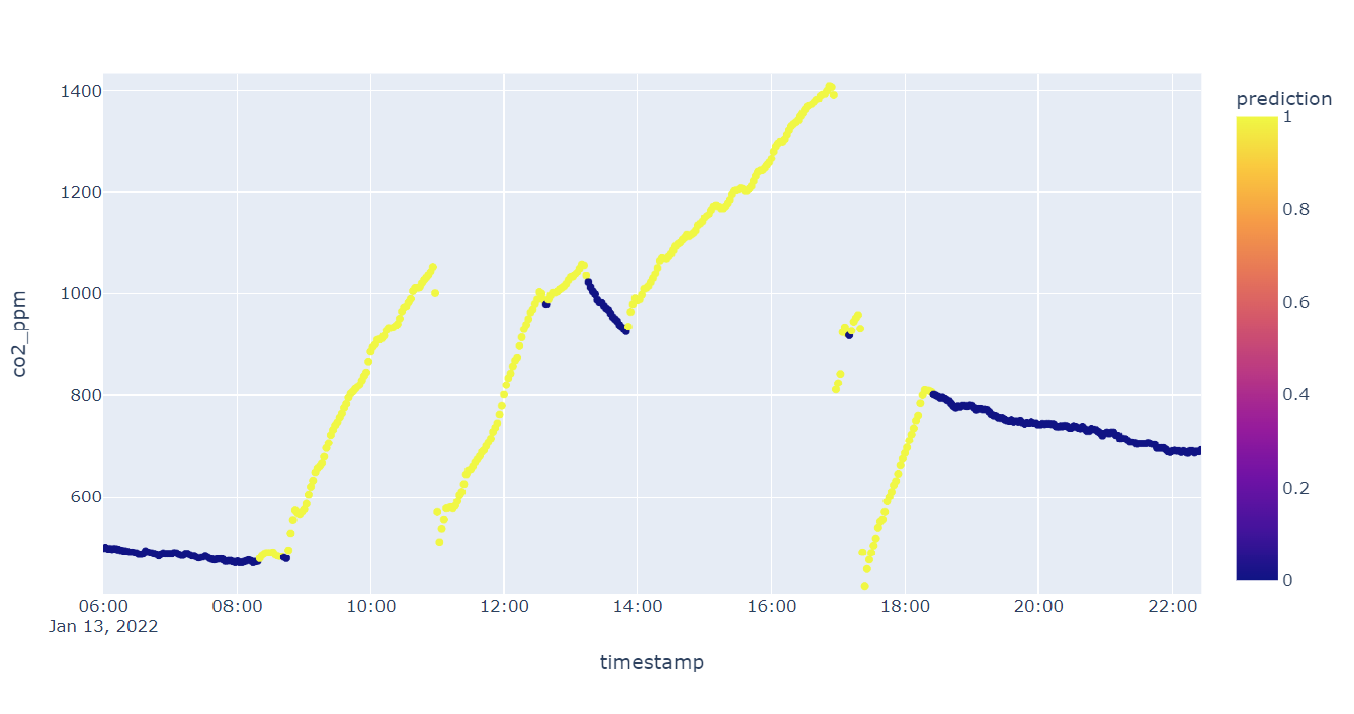
\includegraphics[width=0.9\textwidth]{pic/nov23_predicted.png}
    \caption{Erwartungsberechnung des 13. Januar}
    \label{fig:nov23_pred}
\end{figure}

Dieses Ergebnis konnte über weitere Kombinationen verschiedener Räume und Modelle weiterhin
bestätigt und repliziert werden. 

\newpage
Die Tatsache, dass die Genauigkeiten aller Modelle so nah beieinander 
liegen, rührt daher, dass dieses Datenset ein typisches Klassifizierungsproblem darstellt,
wodurch die sich wiederholenden Schemata in den CO2-Werten von einer Vielzahl von Algorithmen schnell 
erkannt und verarbeitet werden können.

Beim Tuning der ausgewählten Modelle wurden als Parameter-Optionen ausschließlich Werte gewählt, die nicht 
den Standardwerten der Modelle entsprechen. Somit sollte das GridSearchCV-Modul ausschließlich in der Menge 
von Parametern nach Möglichkeiten suchen, die nicht den Standard-Einstellungen entsprechen.

\begin{figure}[h]
    \centering
    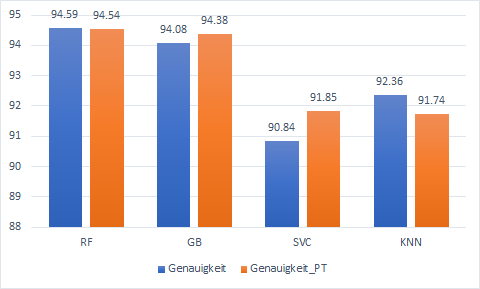
\includegraphics[width=0.6\textwidth]{pic/param_eval.png}
    \caption{!!PLACEHOLDER-GRAFIK!! Ergebnisse des Parameter Tuning}
    \label{fig:PT_eval}
\end{figure}

Es ist zu sehen, dass das Parameter Tuning die Genauigkeit der Modelle im erwarteten Rahmen erhöht oder 
verringert hat. Dies bestätigt die Annahme, dass dieser Anwendungsfall ein typisches Klassifizierungsproblem 
darstellt, weshalb die Modelle nicht mehr maßgeblich verbessert werden können. Der Schritt des Parameter Tunings 
sollte trotzdem grundsätzlich immer durchgeführt werden, um zu erkennen, ob man durch eine einfache Änderung 
der Parameter eine Verbesserung des Modells erzielen kann.\\

\newpage
Zusätzlich wurden die \textit{ROC-Curves} (ROC: englisch für \textit{receiver operating characteristic} bzw. 
deutsch Operationscharakteristik)
der True- und False-Positives gegeneinander gezeichnet, um zu erkennen, 
inwiefern die Ergebnisse zufällig oder errechnet sind.\\\\
Der Optimalwert wird hier durch in der grünen Kurve gezeigt, welche den Fall darstellt, 
dass das Modell die Labels immer richtig berechnet und es nie zu Fehleinschätzungen kommt.\\
Liegt ein Modell näher an der schwarzen Diagonale in der Mitte bedeutet das, dass True- und 
False-Positives jeweils 50\% der Ergebnismenge ausmachen. 
Das Modell liegt dann genauso oft richtig, wie es Fehleinschätzungen trifft. 
Je näher die einzelnen Modelle an der schwarzen Linie liegen, desto weniger aussagefähig sind sie. 

\begin{figure}[h]
    \centering
    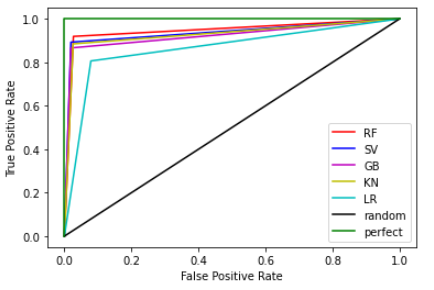
\includegraphics[width=0.7\textwidth]{pic/roc_curves.png}
    \caption{ROC-Curves aller Modelle}
    \label{fig:Roc_curves}
\end{figure}

Man sieht in \ref{fig:Roc_curves}, wie alle Modelle sehr ähnliche Ergebnisse aufweisen. Keines der Modelle weist Anzeichen 
dafür auf, dass Ergebnisse wegen Underfitting erraten werden. Alle Modelle zeigen eine hohe Rate von True-Positives und
sind somit in den meisten Fällen in der Lage, aus den Input-Werten das richtige Ergebnis für die Präsenz abzuleiten.  

\newpage

\subsection{Umgang mit fehlenden Präsenz-Labels}
Da zur Auswertung auch eine große Menge an Datensätzen ohne Präsenz-Label zur Verfügung stand, konnte die 
Qualität der Ergebnisse für diese Datensets nicht rechnerisch quantifiziert werden. Die Ergebnisse
sind hierbei aufgrund der fehlenden Label lediglich augenscheinlich zu bewerten, da eine mathematische
Berechnung der Genauigkeit nicht möglich ist.\\
In diesem Kontext stellt sich die Frage, inwiefern ein auf einen Büroraum trainiertes Modell auch richtige
Erwartungen für einen Wohnraum treffen kann.
Da das Modell unter anderem auf eine Erkennung der aktuellen Tageszeit trainert wird, muss geprüft
werden, inwiefern ein solches Modell auch Aussagen über CO2-Werte treffen kann, dessen Veränderungen außerhalb
der bisher trainierten Arbeitszeiten von etwa 7 Uhr morgens bis 17 Uhr nachmittags liegen. 
Außerdem ist der Wohnraum in der Regel deutlich größer als ein Büro und weist in diesem Fall eine größere Anzahl 
anwesender Personen auf, wodurch sich die ermittelten Deltas der CO2-Werte erheblich von denen der Büroräume 
unterscheiden.\\
Eines der Datensets zeichnete kontinuierliche Werte aus einem Wohnzimmer auf, in dem sich über einen 
Tag hinweg maximal drei Personen befanden. Die Zeiträume, zu denen in diesem Wohnzimmer anhand der CO2-Werte
Anwesenheit zu erkennen war, unterschieden sich deutlich von denen der Datensets der FH Aachen. Die 
starken Anstiege des CO2-Wertes waren bei diesem Datenset viel mehr über den Tag verteilt, wodurch sich die 
Datenreihe für diesen Test besonders anbot.

\begin{figure}[h]
    \centering
    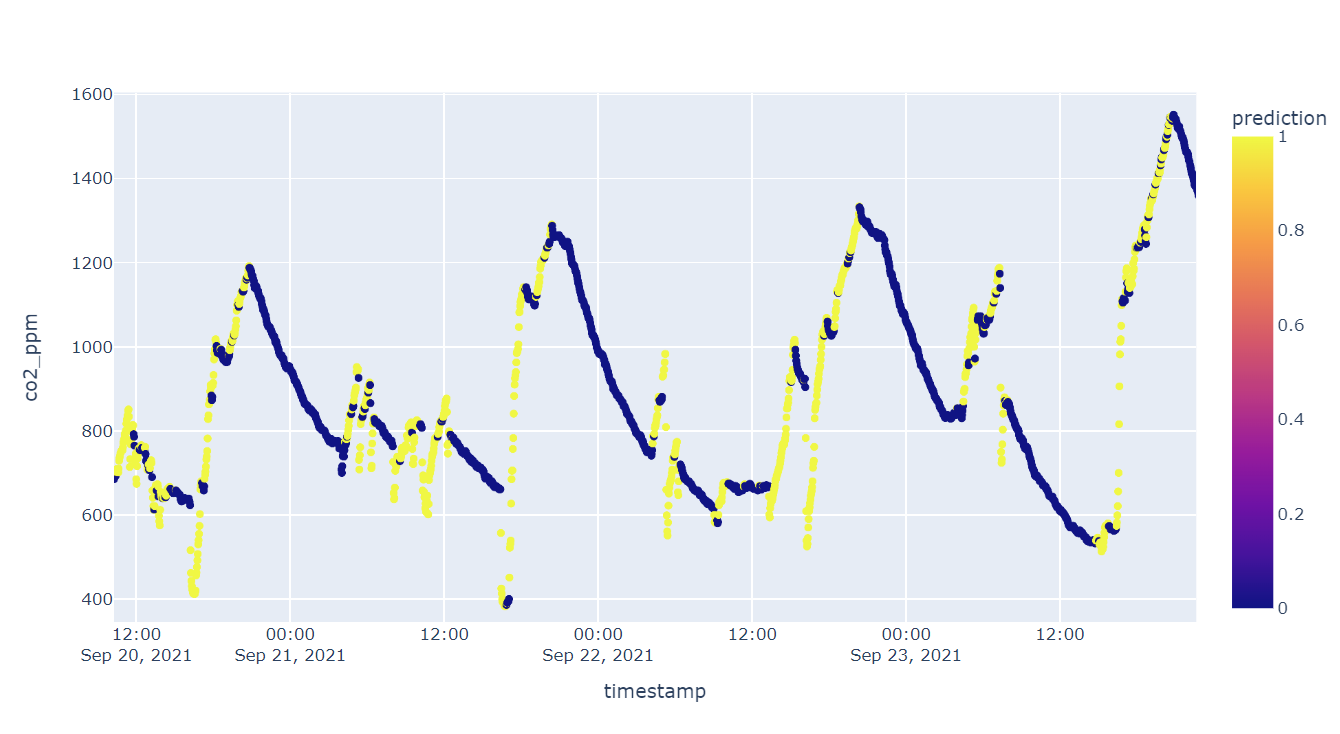
\includegraphics[width=0.95\textwidth]{pic/h217_predicting_livingroom.png}
    \caption{Büroraum-Modell trifft Erwartungen für Wohnzimmer}
    \label{fig:pred_livingroom}
\end{figure}

Auch hier wurden mit den errechneten Anwesenheitswerten des Modells die Einfärbungen der einzelnen Datenpunkte 
vorgenommen. 
Wie in \ref{fig:pred_livingroom} anhand der Einfärbung zu erkennen ist, liegt die Vermutung nahe, dass das Modell 
auch unabhängig von der Tageszeit und den bekannten Gegebenheiten eines normalen Arbeitstages Anwesenheit 
erkennen kann. Vor allem deutliche Anstiege und Abfälle zeigen sich merklich durch kontinuierliche gelbe bzw. 
blaue Einfärbung.
\newpage

\subsection{Neuronale Netzwerke}
Die beiden implementierten neuronalen Netze konnten eine ähnliche Leistung wie die bereits oben genannten 
Algorithmen erzielen. Beide Modelle wurden über so viele Iterationen (Epochen) trainiert, bis ersichtlich war,
dass die Genauigkeit gegen einen Wert konvergiert. Zur Auswertung wurden hier die \textit{Accuracy-} und 
\textit{Loss}-Funktionen genutzt. Die Genauigkeit beschreibt wie bei den anderen Modellen das Verhältnis
zwischen richtigen und falschen Berechnungen.\\
Die Loss-Funktion hingegen gibt die Abweichung einer Schätzung zum tatsächlichen Wert an. Diese beiden Werte 
werden nach jeder Epoche ausgewertet, wobei zunächst der Erfolg während des Trainigs als \textit{train}
angegeben wird und danach das Modell an einem zufälligen Teil des Validierungssets \textit{val} getestet wird.
Liegen diese beiden Kurven nah beieinander, kann dies als ein klares Anzeichen für ein funktionierndes Modell ohne 
Over- oder Underfitting gewertet werden, da sowohl beim Training als auch bei der Validierung die Genauigkeiten 
Ähnlichkeiten aufweisen, während zugleich die Loss-Funktion minimiert wird.

\begin{figure}[h]
    \centering
    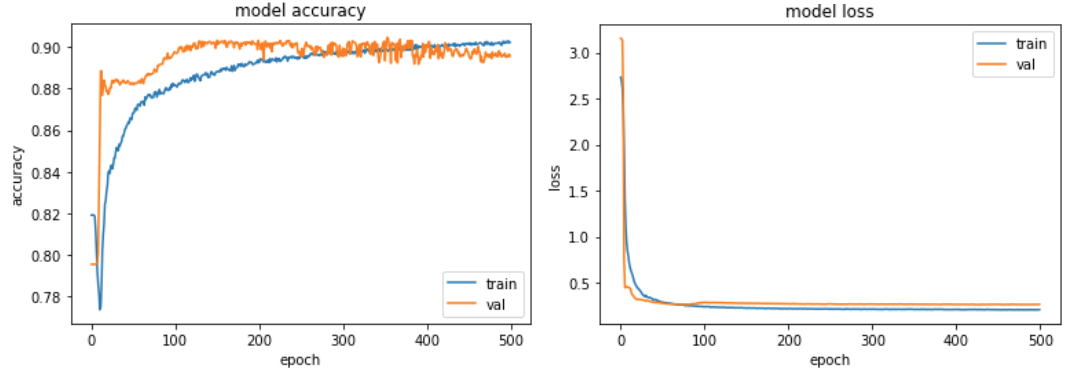
\includegraphics[width=0.9\textwidth]{pic/eval_NN.png}
    \caption{Ergebnisse des NN}
    \label{fig:eval_NN}
\end{figure}

\begin{figure}[h]
    \centering
    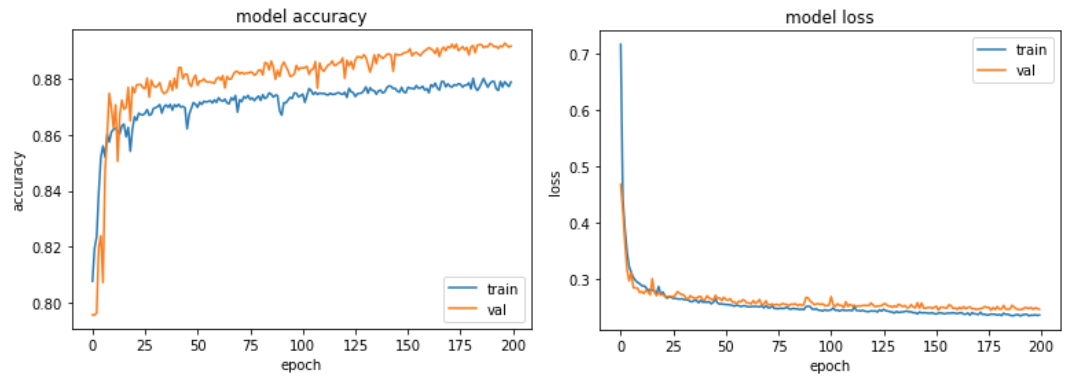
\includegraphics[width=0.9\textwidth]{pic/eval_LSTM.png}
    \caption{Ergebnisse des LSTM}
    \label{fig:eval_LSTM}
\end{figure}

Wie \ref{fig:eval_NN} und \ref{fig:eval_LSTM} zeigen, weisen beide Arten neuronaler Netzwerke diese Eigenschaften auf. Die Genauigkeiten beider Modelle
konvergierten auch nach verschiedenen Epochen-Werten etwa bei 89\%.

\subsection{Clustering Modelle}
Von allen benutzten Algorithmen ergaben sich bei den Clustering Modellen die größten Schwierigkeiten bei der 
Klassifikation des Datensets. 
Während die Genauigkeit bei der Erwartungsberechnung von Abwesenheit bei 94\% lag, konnte das
K-Means-Modell Anwesenheiten nur zu 50\% erkennen, was bedeutet, dass das Modell das Ergebnis errät, anstatt
es zuverlässig zu berechnen. \\
Wegen der Unausgeglichenheit des Datensets sind ca. zwei Drittel des Datensets sehr einfach zu 
klassifizieren, da es im ganzen Datenset nie Anwesenheiten zwischen ca. 20:00 Uhr und 06:00 Uhr 
gibt. Bei diesem Teil der Daten wies das Modell eine hohe Genauigkeit von 94\% auf. So werden also ca. 67\% des 
Datensets mit enorm hoher Genauigkeit klassifiziert.\\
Selbst wenn das Modell beim letzten Drittel der Daten, also dem Teil des Datensets bei dem es zwischen
An- und Abwesenheit unterscheiden muss, rät und somit nur mit einer Genauigkeit von 50\% das richtige Label 
errechnet, suggeriert eine daraus resultierende Gesamtgenauigkeit von etwa 80\% ein funktionierendes Modell.
Allerdings zeigt sich hier, warum auch die Gegenüberstellung von True und False Positives in der 
Modellauswertung von entscheidender Wichtigkeit sein kann.\\

\begin{center}
    \begin{table}[h]
        \centering
        \caption{Genauigkeitsauswertung}
        \begin{tabular}{|p{1.5cm}||p{1.8cm}|p{1.5cm}|p{1.5cm}|}
            \hline
            \hfill Präsenz&\hfill Precision &\hfill Recall &\hfill F1\\
            \hline
            \hline
            \hfill 0&\hfill 0.94&\hfill 0.79&\hfill 0.86\\
            \hfill 1&\hfill 0.50&\hfill 0.82&\hfill 0.62\\
            \hline
        \end{tabular}          
        \label{tab:clus}
    \end{table}
\end{center}

Wie anhand der Precision-Score in \ref{tab:clus} zu sehen ist, tritt hier genau der oben beschriebene Fall ein.
Das Modell erkennt Abwesenheiten nahezu perfekt, während die übrigen Anwesenheiten nicht klar erkannt werden.\\
\newpage
Zur genaueren Untersuchung und Veranschaulichung der Ergebnisse hilft eine Dimensionalitätsreduktion, 
bei der das Datenset auf zwei Dimensionen reduziert wurde und An- und Abwesenheiten in einem Graphen darstellt werden.

\begin{figure}[h]
    \centering
    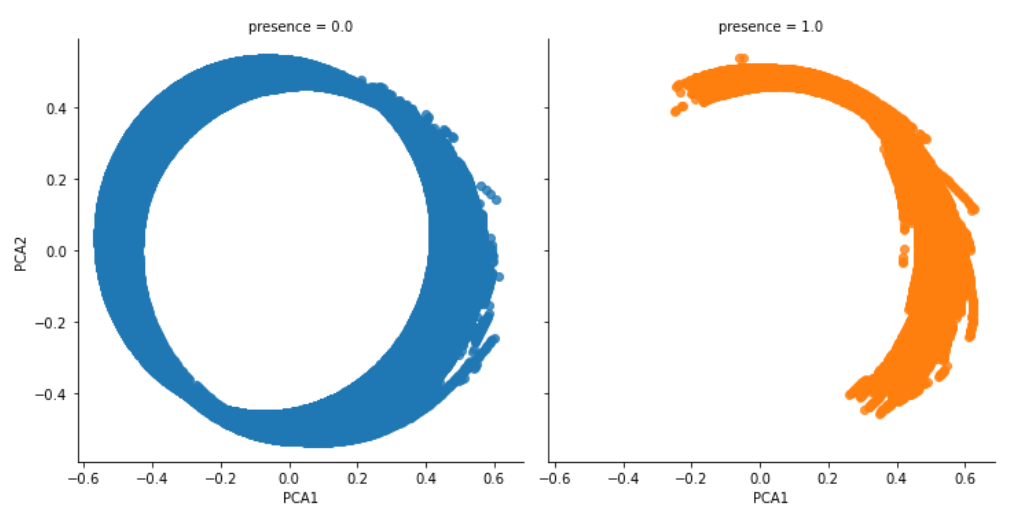
\includegraphics[width=0.85\textwidth]{pic/pca.png}
    \caption{Reduktion des Datensets auf zwei Dimensionen}
    \label{fig:pca}
\end{figure}

Die Menge der Anwesenheiten (orange) ist in \ref{fig:pca} nahezu identisch mit der rechten Teilmenge der 
Abwesenheiten (blau). 
Das heißt, dass alle Datenpunkte, die in der linken Hälfte des blauen Datensets liegen, sehr einfach klassifiziert 
werden können.\\
Legt man beide Datensets übereinander, ist es nun ohne die Einfärbung nahezu unmöglich zwischen An- und 
Abwesenheit zu unterscheiden.\\

\begin{figure}[h]
    \centering
    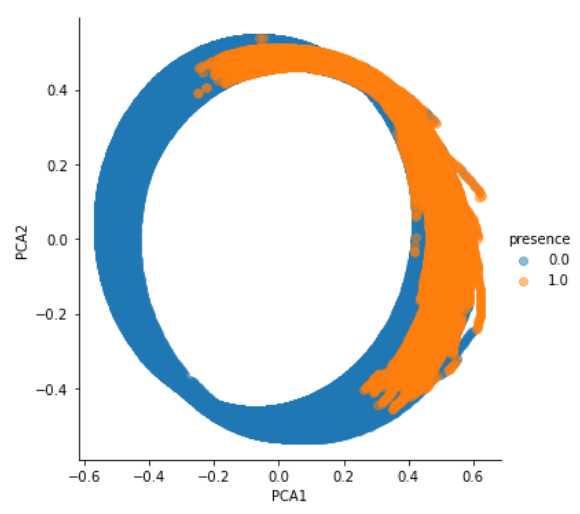
\includegraphics[width=0.5\textwidth]{pic/pca1.png}
    \caption{Datenreduktion ohne Trennung}
    \label{fig:pca1}
\end{figure}

Da die Datenpunkte im rechten Teilbild kaum zu unterscheiden sind, schafft es das Modell nicht, An- und Abwesenheit
während eines Arbeitstages zu unterscheiden. Währenddessen sind die Abwesenheiten im linken Teilbild sehr einfach
zu klassifizieren.
Diesen Sachverhalt spiegelt auch die Auswertung des \textit{Classification Report} in Tabelle \ref{tab:clus} wieder.\\
%Das Erkennen von Abwesenheit im linken Teilbild von \ref{fig:pca1} ist nun erheblich einfacher, als die Trennung 
%zwischen An- und Abwesenheit im rechten Teilbild. 

\clearpage
\chapter{\textbf{Zusammenfassung und Ausblick}}\label{zusammenfassung}
%\addtocontents{toc}{\vspace{0.8cm}}

\section{CO2 als Anwesenheitsindikator}
Die Genauigkeit aller Modelle bei der Präsenzerkennung während der gesamten Durchführungsphase des Projektes 
lag zwischen 88\% bei neuronalen Netzwerken und 95\% bei den Klassifizierungsalgorithmen. 
Die Beziehung zwischen der aktuellen Tageszeit und dem CO2-Gehalt der Luft konnte erfolgreich bestätigt 
werden. Resultate vorangegangener Forschung unterstützen dieses Ergebnis ebenfalls\footnote[1]{\cite{IPPR}}.\\
Weiterhin konnte gezeigt werden, dass alle Modelle zusätzlich in der Lage sind, menschliche Präsenz außerhalb
der trainierten Uhrzeiten korrekt zu erkennen, wenn die Modelle mit Deltas zu Vergangenheitswerten des 
CO2-Gehalts trainiert werden. Die Präsenzerkennung ist also vollständig unabhängig von den Umständen des
Trainingssets und kann sowohl für andere Räume, als auch zu anderen Tageszeiten effektiv genutzt werden. 
Der CO2-Gehalt der Luft kann somit als geeigneter Indikator für menschliche Präsenz in Innenräumen angesehen 
werden.\\\\
Zudem wurde gezeigt, dass der Einsatz von CO2-Sensoren bei Gebäudeautomatisierungssystemen zweckmäßig ist.
Ein weiterer Vorteil besteht darin, dass diese kostengünstig und leicht zu implementieren sind.


\section{Mögliche Verbesserungen}
Die Genauigkeit von Machine Learning Modellen kann allgemein durch die Hinzugabe von mehr Daten in ein Modell 
verbessert werden. \\
Da der Datenbestand, auf die sich diese Arbeit stützt, über die Bearbeitungszeit des Projektes 
kontinuierlich vergrößert wurde, wuchs damit auch die Anzahl an Anhaltspunkten für Zusammenhänge zwischen den 
Datenfeldern stetig an. Besonders nützlich wäre das Sammeln von Messdaten über ein oder mehrere Jahre hinweg.
Somit hätten die Modelle eine Chance, Gewohnheiten in z.B. Urlaubstagen, Feiertagen oder auch wiederkehrenden
Meetings korrekt einzuordnen, sodass Gebäudeautomatisierungssysteme ein Maximum an Komfort und Energieeffizienz
herstellen können.\\\\
Die Anwendung eines Modells auf andere Räume lies die Vermutung zu, dass diese Art von Präsenzerkennung das 
Potential aufweist, anhand eines Traningssets auch eine Vielzahl anderer Datensets klassifizieren zu können.
Durch Aufzeichnung von Daten aus anderen Räumen könnte diese Vermutung genauer untersucht werden.  \\\\

\newpage

Da Infrarotsensoren inhärent nicht in der Lage sind kontinuierliche Präsenz zu erkennen, wenn sich die Personen
im Raum nicht bewegen, kam es innerhalb des Datensets immer wieder zu kleinen Messfehlern, die durch Gruppierung
und Durchschnittsberechnung der Präsenzwerte behoben werden mussten. Es ist klar davon auszugehen, dass eine 
genauere Datenlage auch die Qualität der trainierten Modelle steigern würde.\\
Zusätzlich existierten im Datenset durch seltene Probleme mit der Hardware längere Datenreihen mit falschen 
Labelwerten, welche während der Bearbeitung ausgeschlossen werden mussten. Da sich dadurch die für das Training 
geeignete Datenmenge verringerte, ist auch hier davon auszugehen, dass das Aussortieren dieser Werte
mit einer Verringerung der Modellqualität einherging. 


% Nachspann
%\nocite{Segmentation} % Quelle wird nicht im Text erwähnt -> Quellenverzeichnis
%\nocite{ImageAttack}
% Weitere quellen müssen in 'bib/quellen.bib' eingetragen werden
% !!! -> BibTex ausführen! Sonst tauchen die Quellen nicht im Verzeichnis auf.
%\nocite{Segmentation1}
\nocite{Handbook}
\nocite{CDHOC}
\nocite{DecTrees}
\nocite{FScaling}
\nocite{ParTuning}
% Quellenverzeichnis
\clearpage
%\bibliographystyle{alpha}
\bibliographystyle{apalike}
\bibliography{./bib/quellen}
%\addbibresources{./bib/quellen}
\addcontentsline{toc}{chapter}{Quellenverzeichnis}
%\addtocontents{toc}{\vspace{0.8cm}}

% Abkürzungsverzeichnis
\clearpage
\markright{Abkürzungsverzeichnis}
\clearpage
\chapter*{Abkürzungsverzeichnis}\label{abkuerzungsverzeichnis}
\addcontentsline{toc}{chapter}{Abkürzungsverzeichnis}
\begin{acronym}[YTM]
\setlength{\itemsep}{-\parsep}

\acro{randomforest}[$RFC$]{\hspace{1cm}Random Forest Classifier}
\acro{svc}[$GBC$]{\hspace{1cm}Gradient Boosting Classifier}
\acro{svc}[$SVC$]{\hspace{1cm}Support Vector Classifier}
\acro{lr}[$LR$]{\hspace{1cm}Logistic Regression}
\acro{knn}[$KNN$]{\hspace{0.825cm}K-Nearest-Neighbours}
\acro{lstm}[$LSTM$]{\hspace{0.625cm}Long Short Term Memory}
\acro{hadoop}[$HDFS$]{\hspace{0.625cm}Hadoop Distributed File System}
\acro{iqr}[$IQR$]{\hspace{1cm}Interquartile Range}
\acro{TP}[$TP$]{\hspace{1cm}True Positive}
\acro{FP}[$FP$]{\hspace{1cm}False Positive}
\acro{TN}[$TN$]{\hspace{1cm}True Negative}
\acro{FN}[$FN$]{\hspace{1cm}False Positive}
\acro{FV}[$FV$]{\hspace{1cm}Feature Vektor}
\acro{ROC}[$ROC$]{\hspace{1cm}Reciever Operating characteristic}





%\acro{Nu}[$Nu$]{\hspace{1cm}Nußelt-Zahl}
%\acro{nu_luft}[$\nu_{Luft}$]{\hspace{1cm}Kinematische Viskosität von Luft}
%\acro{Pr}[$Pr$]{\hspace{1cm}Prandtl-Zahl}
%\acro{Q}[$\dot Q$]{\hspace{1cm}Wärmestrom}
%\acro{Ra}[$Ra$]{\hspace{1cm}Rayleigh-Zahl}
%\acro{rho_luft}[$\rho_{Luft}$]{\hspace{1cm}Dichte von Luft}
%\acro{temperatur}[$T$]{\hspace{1cm}Temperatur}
%\acro{umgebungstemperatur}[$T_{\infty}$]{\hspace{1cm}Umgebungstemperatur}

\end{acronym}
%\addtocontents{toc}{\vspace{0.8cm}}

% Abbildungsverzeichnis
\clearpage
\addcontentsline{toc}{chapter}{Abbildungsverzeichnis}
\listoffigures
%\addtocontents{toc}{\vspace{0.8cm}}

% Tabellenverzeichnis
\clearpage
\addcontentsline{toc}{chapter}{Tabellenverzeichnis}
\listoftables
\addtocontents{toc}{\vspace{0.8cm}}

% Anhaenge
\addcontentsline{toc}{chapter}{Anhang}
\appendix
%\input{./app/Anwesenheitsanalyse.py}
%\input{./app/createModel.py}
%\input{./app/drill.py}
%\input{./app/modelTuning.py}
%\input{./app/prepareData.py}
%input{./app/validation.py}
\lstset{ 
  backgroundcolor=\color{white},   % choose the background color; you must add \usepackage{color} or \usepackage{xcolor}; should come as last argument
  basicstyle=\footnotesize,        % the size of the fonts that are used for the code
  breakatwhitespace=false,         % sets if automatic breaks should only happen at whitespace
  breaklines=true,                 % sets automatic line breaking
  captionpos=b,                    % sets the caption-position to bottom
  deletekeywords={...},            % if you want to delete keywords from the given language
  escapeinside={\%*}{*)},          % if you want to add LaTeX within your code
  extendedchars=true,              % lets you use non-ASCII characters; for 8-bits encodings only, does not work with UTF-8
  firstnumber=1,                   % start line enumeration with line 1000
  frame=single,	                 % adds a frame around the code
  keepspaces=true,                 % keeps spaces in text, useful for keeping indentation of code (possibly needs columns=flexible)
  %keywordstyle=\color{blue},       % keyword style
  language=Octave,                 % the language of the code
  morekeywords={*,...},            % if you want to add more keywords to the set
  numbers=left,                    % where to put the line-numbers; possible values are (none, left, right)
  numbersep=10pt,                   % how far the line-numbers are from the code
  rulecolor=\color{black},         % if not set, the frame-color may be changed on line-breaks within not-black text (e.g. comments (green here))
  showspaces=false,                % show spaces everywhere adding particular underscores; it overrides 'showstringspaces'
  showstringspaces=false,          % underline spaces within strings only
  showtabs=false,                  % show tabs within strings adding particular underscores
  stepnumber=1,                    % the step between two line-numbers. If it's 1, each line will be numbered
  tabsize=2,	                   % sets default tabsize to 2 spaces
  title=\lstname                   % show the filename of files included with \lstinputlisting; also try caption instead of title
}
\chapter{Quellcode}
Hier steht der Quellcode
%\lstinputlisting[language=Python]{app/Anwesenheitsanalyse.py}
%\lstinputlisting[language=Python]{app/createModel.py}
%\lstinputlisting[language=Python]{app/drill.py}
%\lstinputlisting[language=Python]{app/modelTuning.py}
%\lstinputlisting[language=Python]{app/prepareData.py}
%\lstinputlisting[language=Python]{app/validation.py}
%\begin{enumerate}
%      \item Source 1
%      \item Source 2
%\end{enumerate}

% Anhänge im Ordner 'app' ablegen

%\includepdf[pages=1-4]{./app/Datenblatt1.pdf} % Datei mit 4 Seiten
%\includepdf[pages=1]{./app/Datenblatt2.pdf} % Datei mit einer Seite

\chapter{Rohdatenvisualisierungen}
\begin{enumerate}
      \item Graustufen
      \item Verteilungen
\end{enumerate}
\end{document}
